%Update 09/02/2023
% Changelog
% v. 1.0 limiti
% v. 2.0 nuovo stile
% v. 3.0 derivate fino a punti di non derivabilità
%%%%%%%%%%%%%%%%%%%%%%%%%%%%%%%%%%%%%%%%%%%%%%%%%%%%%%%%%%%%%%%%%%%%%%%%%%%%%%%%%%%%%%%%
\documentclass{book}     %type of document
\usepackage[utf8]{inputenc} %for text encoding
\usepackage{lambdatex} 

\usepackage{tasks}
\usepackage{exsheets}

\makeatletter
\renewcommand*\env@cases[1][1.2]{%
  \let\@ifnextchar\new@ifnextchar
  \left\lbrace
  \def\arraystretch{#1}%
  \array{@{}l@{\quad}l@{}}%
}
\makeatother

\title{Analisi 1}
\author{Davide Borra}
\date{}
\makeatletter
\let\runauthor\@author
\let\runtitle\@title
\renewcommand{\chaptermark}[1]{\markboth{#1}{}}
\renewcommand{\sectionmark}[1]{\markright{#1}}
\renewcommand{\footrulewidth}{0.4pt}

\everymath{\displaystyle}

\begin{document}

\lhead{}
\chead{}
\rhead{Indice}
\rfoot{\runauthor}

\begin{titlepage}
    \newgeometry{left=3cm, right=3cm, bottom=2cm, top =3cm} 
    \pagestyle{empty}
    \begin{center}
        \vspace*{\fill}
        \vspace{0.5cm}
        \textbf{\Huge \runtitle}\\\vspace{5mm}
        \textsc{\Large \runauthor}
        \vspace{5cm}
    \end{center}
    \vspace*{\fill}
    v. 3.0\\
    \rule{0.8\linewidth}{0.5mm}\\
    {\footnotesize\href{mailto:davide.borra@studenti.unitn.it}{davide.borra@studenti.unitn.it} - \href{http://davideborra.github.io}{davideborra.github.io}}
    \restoregeometry
\end{titlepage}
\thispagestyle{empty}
\frontmatter
    \tableofcontents
    \creativecommons
\mainmatter
\lhead{Analisi 1}
\chead{}
\rhead{\leftmark\ - \rightmark}
\rfoot{\runauthor}


\chapter{Limiti}
\section{Intervalli in $\mathbb{R}$}
\begin{boxdef}
    Un insieme $A \subset \R$ si dice \textbf{intervallo} se corrisponde ad una semiretta (\textbf{illimitato}) o ad un segmento (\textbf{limitato}) della retta reale
\end{boxdef}
Inoltre:
\begin{itemize}
    \item si dice \textbf{chiuso} se gli estremi sono inclusi nell'intervallo;
    \item si dice \textbf{aperto} se gli estremi sono esclusi nell'intervallo.
\end{itemize}
Gli intervallo limitati corrispondono a segmenti di retta reale di estremi $a$ e $b$ ($b>a$), lunghezza $b-a$ (detta \textbf{ampiezza} dell'intervallo), \textbf{centro} $\frac{b+a}{2}$ e \textbf{raggio} $\frac{b-a}{2}$.
\subsection{Intorni}
\begin{boxdef}
    Dato numero reale $x_0$, un intorno completo di $x_0$ è un qualunque intervallo aperto contenente $x_0$ \[I(x_0)=]x_0-\delta_1;x_0+\delta_2[ ~~~~~~ (\text{con }\delta_1, \delta_2 \in \R_0^+ )\]
\end{boxdef}
\begin{itemize}
    \item \textbf{Intorno destro}: $I^+(x_0)=]x_0;x_0+\delta[$
    \item \textbf{Intorno sinistro}: $I^-(x_0)=]x_0-\delta;x_0[$
\end{itemize}
\subsubsection{Intorni circolari}
    \begin{boxdef}
        Dati un numero reale $x_0$ e un numero reale positivo $\delta$, un intorno circolare di $x_0$ di raggio $\delta$ è l'intervallo aperto $I_\delta (x_0)$ di centro $x_0$ e raggio $\delta$ \[I_\delta(x_0)=]x_0-\delta;x_0+\delta[\]
    \end{boxdef}
\subsubsection{Intorni di $\infty$}
\begin{boxdef}
    Dati due numeri reali $a$ e $b$ con $a<b$ si definisce 
    \begin{itemize}
        \item \textbf{intorno di $-\infty$} un qualsiasi intervallo illimitato inferiormente $]-\infty;a[$
        \item \textbf{intorno di $+\infty$} un qualsiasi intervallo illimitato superiormente $]b;+\infty[$
        \item \textbf{intorno di $\infty$} l'unione di un intorno di $-\infty$ e di un intorno di $+\infty$: $]-\infty;a[\  \cup\  ]b;+\infty[$
    \end{itemize}
\end{boxdef}
\subsection{Insiemi limitati e illimitati, maggiorante, minorante, estremi, massimo, minimo.}
È possibile definire come limitati/illimitati anche insiemi che non sono intervalli. 
\begin{boxdef}
    [Insiemi limitati]
    Un insieme $X\subseteq R$ non vuotoè detto
    \begin{itemize}
        \item \textbf{superiormente limitato} se è possibile determinare un qualsiasi numero reale $\alpha$ tale che $\forall x \in X, x\leq \alpha$. $\alpha$ è detto \textbf{maggiorante} di $X$.
        \item \textbf{inferiormente limitato} se è possibile determinare un qualsiasi numero reale $\beta$ tale che $\forall x \in X, x\geq \beta$. $\beta$ è detto \textbf{minorante} di $X$.
        \item \textbf{limitato} se è limitato sia superiormente che inferiormente.
    \end{itemize}
\end{boxdef}
\begin{boxdef}
    [Insiemi illimitati]
    Un insieme $X\subseteq R$ non vuoto è detto 
    \begin{itemize}
        \item \textbf{superiormente illimitato} se $\forall \alpha \in \R, \exists x \in X : x>\alpha$
        \item \textbf{inferiormente illimitato} se $\forall \beta \in \R, \exists x \in X : x<\beta$
        \item \textbf{illimitato} si è illimitato sia inferiormente che superiormente.
    \end{itemize}
\end{boxdef}

Se un insieme è limitato superiormente/inferiormente è possibile definire minimo e massimo è possibile quindi definire massimo e minimo di un insieme (attenzione, non è detto che tutti gli insiemi limitati ammettano massimo/minimo.)
\begin{boxdef}[Massimo]
    Dati un insieme $X\subseteq R$ e un numero reale $M$, esso si dice \textbf{massimo} di $X$ se 
    \begin{enumerate}[label={\roman*)}]
        \item $\forall x\in X, M\geq x $ (è maggiorante)
        \item $M\in X$ (appartiene all'insieme).
    \end{enumerate}
    Si indica $M=\max X$.
\end{boxdef}
\begin{boxdef}[Minimo]
    Dati un insieme $X\subseteq R$ e un numero reale $m$, esso si dice \textbf{minimo} di $X$ se 
    \begin{enumerate}[label={\roman*)}]
        \item $\forall x\in X, m\leq x $ (è minorante)
        \item $m\in X$ (appartiene all'insieme)
    \end{enumerate}
    Si indica $M=\min X$.
\end{boxdef}
Tuttavia non è possibile determinare massimo e minimo per, ad esempio, intervalli aperti. Abbiamo quindi bisogno di qualcos'altro che funzioni sempre, definiamo quindi gli estremi inferiore e superiore di un insieme.

\begin{boxdef}[Estremo superiore]
    Dato un insieme $X$ superiormente limitato, si dice \textbf{estremo superiore} di $X$ il minimo dei suoi maggioranti
    \[\inf X = \min\{M\in \R : M \text{ è maggiorante di }X\}\]
    Se $X$ è superiormente illimitato, si definisce $\sup X = +\infty$.
\end{boxdef}
\paragraph{Caratterizzazione di $\sup X$}
Si dimostra che la seguente definizione di $\sup$ è equivalente alla precedente: dato un insieme $X$ superiormente limitato, un numero reale $M$ si dice estremo superiore di $X$ se e solo se 
\begin{enumerate}[label={\roman*)}]
    \item $\forall x\in X, M\geq x $ (è maggiorante)
    \item $\forall \varepsilon >0 \exists x\in X: x>M-\varepsilon$ (è il minore dei maggioranti)
\end{enumerate}

\begin{boxdef}[Estremo inferiore]
    Dato un insieme $X$ inferiormente limitato, si dice \textbf{estremo inferiore} di $X$ il massimo dei suoi minoranti
    \[\inf X = \max\{m\in \R : m \text{ è minorante di }X\}\]
    Se $X$ è inferiormente illimitato, si definisce $\inf X = -\infty$.
\end{boxdef}
\paragraph{Caratterizzazione di $\inf X$}
Si dimostra che la seguente definizione di $\inf$ è equivalente alla precedente: dato un insieme $X$ inferiormente limitato, un numero reale $m$ si dice estremo inferiore di $X$ se e solo se 
\begin{enumerate}[label={\roman*)}]
    \item $\forall x\in X, m\leq x $ (è minorante)
    \item $\forall \varepsilon >0 \exists x\in X: x<m+\varepsilon$ (è il maggiore dei minoranti)
\end{enumerate}
\subsection{Punti di accumulazione e punti isolati}
\begin{boxdef}[Punto isolato]
    Sia $x_0\in X\subseteq\R$, allora $x_0$ si definisce punto isolato di $X$ se esiste un intorno $I(x_0)$ che non contiene altri elementi di $X$.
\end{boxdef}
\begin{boxdef}[Punto di accumulazione]
    Sia $ X\subseteq\R$, allora $x_0\in \R$ si definisce punto di accumulazione di $X$ se ogni intorno completo $I(x_0)$ contiene altri infiniti elementi di $X$,\\
    \textbf{equivalentemente} se ogni intorno completo $I(x_0)$ contiene almeno un altro elemento di $X$.
\end{boxdef}
\begin{boxdef}[Insieme derivato]
    Dato un insieme $A\subseteq R$, si definisce \textbf{insieme derivato} di $A$, l'insieme $DA$ contenente tutti e soli i suoi punti di accumulazione.
\end{boxdef}
\begin{ex}[
    Dato l'insieme \[A =\left\{x\in \R\;\bigg|\;x =\frac{n + 1}{n}, n\in \N_{ > 0}\right\}\]
    \begin{tasks}(1)
        \task precisare se è limitato,
        \task rappresentarlo graficamente,
        \task determinare $\sup A$ e $\inf A$, specificando se sono massimo e minimo,
        \task indicare punti di accumulazione e punti isolati.
    \end{tasks}
]
     \begin{enumerate}[label=\textit{\alph*)}]
        \item Cominciamo espandendo alcuni elementi dell'insieme
        \[A =\left\{1, \frac{3}{2}, \frac{4}{3}, \frac{5}{4}, \frac{6}{5}, \dots \right\}\]
        Osserviamo facilmente che è limitato inferiormente superiormente
        \item Anche qui calcoliamo i primi elementi, in modo da poterli rappresentare:
        \begin{center}
            \renewcommand{\arraystretch}{1.5}
            \everymath{\textstyle}
            \begin{tabular}[h]{|c||c|c|c|c|c|}
                \hline
                $n$&$1$&$2$&$3$&$4$&$5$\\\hline
                $x$&$2$&$\frac{3}{2}$& $\frac{4}{3}$& $\frac{5}{4}$& $\frac{6}{5}$\\ \hline
            \end{tabular}\\
            \begin{tikzpicture}[line cap=round,line join=round,>=triangle 45,x=1.0cm,y=1.0cm]
                \begin{axis}[
                x=1.0cm,y=1.0cm,
                axis lines=middle,
                ymajorgrids=true,
                xmajorgrids=true,
                xmin=-0.5,
                xmax=10.5,
                ymin=-0.5,
                ymax=3.5,
                xlabel=$n$,
                ylabel=$x$,
                xtick={-0.0,1.0,...,10.0},
                ytick={-0.0,1.0,...,3.0},]
                \clip(-0.5,-0.5) rectangle (10.5,3.5);
                \draw[line width=1.pt,dashed,color=teal,smooth,samples=100,domain=1.0000000399999984:10.5] plot(\x,{((\x)+1)/(\x)+0*sqrt((\x)-1)});
                \draw [line width=1.pt,dashed,color=teal,domain=0.0:10.5] plot(\x,{(--0.5-0.*\x)/0.5});
                \begin{scriptsize}
                \draw [fill=teal] (1.,2.) circle (2.5pt);
                \draw [fill=teal] (2.,1.5) circle (2.5pt);
                \draw [fill=teal] (3.,1.3333333333333333) circle (2.5pt);
                \draw [fill=teal] (4.,1.25) circle (2.5pt);
                \draw [fill=teal] (5.,1.2) circle (2.5pt);
                \draw [fill=teal] (6.,1.1666666666666667) circle (2.5pt);
                \draw [fill=teal] (7.,1.1428571428571428) circle (2.5pt);
                \draw [fill=teal] (8.,1.125) circle (2.5pt);
                \draw [fill=teal] (9.,1.1111111111111112) circle (2.5pt);
                \draw [fill=teal] (10.,1.1) circle (2.5pt);
                \draw [fill=teal] (11.,1.0909090909090908) circle (2.5pt);
                \draw [fill=teal] (12.,1.0833333333333333) circle (2.5pt);
                \draw [fill=teal] (13.,1.0769230769230769) circle (2.5pt);
                \draw [fill=teal] (14.,1.0714285714285714) circle (2.5pt);
                \draw [fill=teal] (15.,1.0666666666666667) circle (2.5pt);
                \end{scriptsize}
                \end{axis}
                \end{tikzpicture}
        \end{center}
        \item Dal disegno si vede chiaramente che \[\sup A = 2 =\max A,\]
        inoltre osserviamo che \[x =\frac{n + 1}{n} =\frac{n}{n} + \frac{1}{n} = 1 + \frac{1}{n}\underset{n\to +\infty}{\xrightarrow{\hspace{1cm}}}1\]
        quindi 
        \[\inf A = 1\qquad\qquad \nexists \min A\]
        \item Osserviamo che qualsiasi punto dell'insieme consideriamo esiste un suo intorno (ad esempio l'intorno circolare di raggio $\textstyle \frac{1}{2}$), per cui tutti i punti dell'insieme sono punti isolati. Osserviamo inoltre che i punti si \say{addensano} intorno a $1$, per cui ogni intorno di $1$ contiene almeno un punto dell'insieme, per cui $x=1$ è un punto di accumulazione per l'insieme $A$.
     \end{enumerate}
\end{ex}
\section{Definizione di limite}
\begin{boxdef}[Definizione unificata di limite]
    Sia $f:X\subset\R\to \R$, $x_0\in \R^\ast$ punto di accumulazione per $X$, allora $l\in \R^\ast$ si dice \underline{limite per $x$ che tende a $x_0$ di $f(x)$} e si scrive
    \[\lim_{x\to x_0}f(x) = l\qquad\qquad\qquad \left(f(x)\underset{x\to x_0}{\xrightarrow{\hspace{1cm}}}l\right)\]
    se
    \[\forall I(l)\ \exists I(x_0) \ :\ f(x)\in I(l)\ \forall x \in I(x_0)\setminus \{x_0\}\]
\end{boxdef}
Definiamo inoltre i limiti destro e sinistro, che si ottengono sostituendo nella definizione precedente a $I(x_0)$, 
\[\begin{array}{lll}
    \text{Limite sinistro:} & \lim_{x \to x_0^-}f(x) = l \qquad &I^-(x_0)\\
    \text{Limite destro:} & \lim_{x \to x_0^+}f(x) = l & I^ +(x_0)
\end{array}\]
Analogamente definiamo i limiti per eccesso e per difetto, che si ottengono sostituendo nella definizione precedente a $I(l)$, 
\[\begin{array}{lll}
    \text{Limite per eccesso:} & \lim_{x \to x_0}f(x) = l^+\qquad &I^ + (l)\\
    \text{Limite per difetto:} & \lim_{x \to x_0}f(x) = l^-  & I^ - (l)
\end{array}\]

Vediamo ora qualche applicazione delle definizioni di limite a casi particolari:
\begin{itemize}
    \item Limite $+\infty$ per $x\to x_0$: $\lim_{x\to x_0}f(x)=+\infty$
    \[\forall M > 0\ \exists \delta > 0\ :\ f(x) > M\ \forall x \in ] x_0 -\delta, x_0 +\delta[\]
    \item Limite finito per $x\to +\infty$: $\lim_{x\to +\infty}f(x)=l$
    \[\forall \varepsilon > 0\ \exists c > 0\ :\ |f(x) - l |< \varepsilon \ \forall x \in ] c, \infty[\]
    \item Limite $+\infty$ per $x\to +\infty$: $\lim_{x\to +\infty}f(x)=+\infty$
    \[\forall M > 0\ \exists c > 0\ :\ f(x) > M\ \forall x \in ] c,\infty[\]
    \item Limite finito per $x\to x_0$: $\lim_{x\to x_0}f(x)=l$
    \[\forall \varepsilon > 0\ \exists \delta > 0\ :\ |f(x) - l |< \varepsilon \ \forall x \in ] x_0 -\delta, x_0 + \delta[\]
\end{itemize}

\begin{ex}[
    Verificare il seguente limite mediante definizione:
    \[\lim_{x\to -\infty}\frac{2x - 1}{x + 1} = 2\]
]
    Cominciamo determinando il dominio: $\dom f = x+1\neq 0\ \Harr\ x\neq -1$. Ora rappresentiamo il grafico della funzione, osserviamo che si tratta di un'omografica con asintoti $y=2$ e $x=-1$:\\
    \begin{center}
        \begin{tikzpicture}[scale=0.8, line cap=round,line join=round,>=triangle 45,x=1.0cm,y=1.0cm]
            \begin{axis}[
            x=1.0cm,y=1.0cm,
            axis lines=middle,
            ymajorgrids=true,
            xmajorgrids=true,
            xmin=-5.5,
            xmax=5.5,
            ymin=-2.5,
            ymax=6.5,
            xtick={-5.0,-4.0,...,5.0},
            ytick={-2.0,-1.0,...,6.0},]
            \clip(-5.5,-2.5) rectangle (5.5,6.5);
            \draw[line width=1.5pt,color=teal,smooth,samples=100,domain=-5.5:-1.1] plot(\x,{(2*(\x)-1)/((\x)+1)});
            \draw[line width=1.5pt,color=teal,smooth,samples=100,domain=-0.9:5.5] plot(\x,{(2*(\x)-1)/((\x)+1)});
            \draw [line width=1.pt,dash pattern=on 3pt off 3pt,color=red] (-1.,-2.5) -- (-1.,6.5);
            \draw [line width=1.pt,dash pattern=on 3pt off 3pt,color=red,domain=-5.5:5.5] plot(\x,{(--2.-0.*\x)/1.});
            \draw [color=teal](-2.5518824196978303,4.217038073385454) node[anchor=north west] {$y=\frac{2x - 1}{x + 1}$};
            \draw (-0.0894460540647984,1.1015799091315117) node[anchor=north west] {$\left(\frac{1}{2},0\right)$};
            \draw (0.01939091237202069,-0.816671624317422) node[anchor=north west] {$(0,-1)$};
            \draw [color=red](-0.9601417855593511,6.121684986029785) node[anchor=north west] {$x=-1$};
            \draw [color=red](4.100777153752737,2.5436697144193627) node[anchor=north west] {$y=2$};
            \begin{scriptsize}
            \draw [fill=black] (0.,-1.) circle (2.0pt);
            \draw [fill=black] (0.5,0.) circle (2.0pt);
            \end{scriptsize}
            \end{axis}
            \end{tikzpicture}
    \end{center}
    Recuperiamo la definizione di limite
    \[\forall \varepsilon > 0\ \exists I( -\infty)\ :\ \left|\frac{2x - 1}{x + 1} - 2\right|<\varepsilon \ \forall x \in I( -\infty)\]
    e svolgiamo la disequazione.
    \[\begin{cases} \left|\frac{2x - 1}{x + 1} - 2\right|<\varepsilon\\x\neq - 1 \end{cases}\qquad \begin{cases}\left|\frac{\cancel{2x} - 1 - \cancel{2x} - 2}{x + 1}\right|<\varepsilon \\ x\neq - 1\end{cases}\]
    \[\begin{cases}[2] -\frac{3}{x + 1} <\varepsilon \\  -\frac{3}{x + 1} >-\varepsilon\\x\neq 0\end{cases}\qquad \begin{cases}[2] \frac{ -3 -\varepsilon x -\varepsilon}{x + 1} < 0 \\  \frac{ -3 +\varepsilon x +\varepsilon}{x + 1} > 0\\x\neq 0\end{cases} \]
    Separando le due disequazioni
    \begin{enumerate}[label={\Roman*)\ \ }]
        \item $\frac{ -3 -\varepsilon x -\varepsilon}{x + 1} < 0$\\
        \begin{tikzpicture}
            \node at (0,0.4) [anchor=west]{$-3 -\varepsilon x -\varepsilon>0$};
            \node at (0,-0.4)[anchor=west]{$x+1>0$};
            \node at (4,0.4)[anchor=west]{$x<-1-\frac{3}{\varepsilon}$};
            \node at (4,-0.4)[anchor=west]{$x>-1$};
            \draw[->] (7.5,1)--(11.5,1);
            \draw (8.75,1)node [above]{$\textstyle-1-\frac{3}{\varepsilon}$}--(8.75,-1);
            \draw (10.25,1) node [above]{$\textstyle-1$}--(10.25,-1);
            \draw[color=red] (7.5, 0.4)--(8.75,0.4) node {$\circ$};
            \draw[color=red, dashed] (8.75, 0.4)--(11.5,0.4);
            \draw[color=red, dashed] (7.5, -0.4)--(10.25,-0.4) node{$\circ$};
            \draw[color=red] (10.25, -0.4)--(11.5,-0.4);
            \node [color=red]at (8.125,-0.8){$\ominus$};
            \node [color=red]at (9.5,-0.8){$+$};
            \node [color=red]at (11,-0.8){$\ominus$};
            \node at (9.5,-1.6){$x <- 1 -\frac{3}{\varepsilon}\ \ \lor\ \ x > 1$};
        \end{tikzpicture}
        \item $\frac{ -3 +\varepsilon x +\varepsilon}{x + 1} > 0$\\
        \begin{tikzpicture}
            \node at (0,0.4) [anchor=west]{$-3 +\varepsilon x +\varepsilon>0$};
            \node at (0,-0.4)[anchor=west]{$x+1>0$};
            \node at (4,0.4)[anchor=west]{$x>-1+\frac{3}{\varepsilon}$};
            \node at (4,-0.4)[anchor=west]{$x>-1$};
            \draw[->] (7.5,1)--(11.5,1);
            \draw (8.75,1)node [above]{$\textstyle-1$}--(8.75,-1);
            \draw (10.25,1) node [above]{$\textstyle-1+\frac{3}{\varepsilon}$}--(10.25,-1);
            \draw[color=red, dashed] (7.5, 0.4)--(10.25,0.4) node{$\circ$};
            \draw[color=red] (10.25, 0.4)--(11.5,0.4);
            \draw[color=red] (7.5, -0.4)--(8.75,-0.4) node {$\circ$};
            \draw[color=red, dashed] (8.75, -0.4)--(11.5,-0.4);
            \node [color=red]at (8.125,-0.8){$\oplus$};
            \node [color=red]at (9.5,-0.8){$-$};
            \node [color=red]at (11,-0.8){$\oplus$};
            \node at (9.5,-1.6){$x <- 1\ \ \lor\ \ x >- 1 +\frac{3}{\varepsilon}$};
        \end{tikzpicture}
    \end{enumerate}
    In conclusione
    \[\begin{cases} 
        x <- 1 -\frac{3}{\varepsilon} \lor x > 1\\
        x <- 1 \lor x >- 1 +\frac{3}{\varepsilon}\\
        x\neq - 1
    \end{cases}\qquad 
    x <- 1 -\frac{3}{\varepsilon} \lor x >- 1 +\frac{3}{\varepsilon}
    \]
    Che contiene un intorno di $-\infty$, $I(-\infty)=\;\left]-\infty, - 1 -\frac{3}{\varepsilon}\right[$. Il limite è quindi verificato.
\end{ex}
\subsection{Asintoti}
\begin{table}[h]
    \centering
    \begin{tabular}{|m{0.25\textwidth}|m{0.4\textwidth}|m{0.25\textwidth}|}
            \hline
            \textbf{Tipologia} & \textbf{Condizioni} & \textbf{Asintoto}\\
            \hline
            Asintoto verticale&  \[\lim_{x\rightarrow x_0} f(x) = \infty\] & \[x= x_0\]\\\hline
            Asintoto orizzontale & \[\lim_{x\rightarrow \infty} f(x) = l\] & \[y=l\]\\ \hline
            Asintoto obliquo & \[\textnormal{CN: }\lim_{x\rightarrow\infty}f(x) = \infty\]
            \[m=\lim_{x\rightarrow\infty}\frac{f(x)}{x} \qquad ~q=\lim_{x\rightarrow\infty}\left[f(x)-mx\right]\] & \[y=mx+q\] \\ \hline
    \end{tabular}
\end{table}
    \textbf{NB.:} Una funzione può avere anche infiniti asintoti verticali, ma al massimo due tra asintoti orizzontali e asintoti obliqui (uno destro e uno sinistro).
\section{Continuità}
\begin{boxdef}
    Sia $f(x)$ una funzione definita in un intervallo $]a;b[$ e $x_0$ un punto appartenente all'intervallo. $f(x)$ è continua in $x_0$ se e solo se \[\lim_{x\to x_0}f(x)=f(x_0)\]
    La funzione è inoltre continua in $]a;b[$ se è continua in ogni punto $x_0$ dell'intervallo.
\end{boxdef}
Si parla anche di funzioni
\begin{itemize}
    \item \textbf{continue da destra} $x_0$ quando $\lim_{x\to x_0^+}f(x)=f(x_0)$
    \item \textbf{continue da sinistra} $x_0$ quando $\lim_{x\to x_0^-}f(x)=f(x_0)$
\end{itemize}
\section{Primi teoremi sui limiti}
\textbf{N.B.:} I seguenti teoremi valgono per ogni tipologia di limite, sia finito che infinito, e in ogni intorno, sia di un numero reale (anche destro e sinistro) sia di infinito.
    \subsection{Teorema di unicità del limite}
        \begin{shadedTheorem}[Unicità del limite]
            Se una funzione $f(x)$ ha limite finito per $x$ che tende a $x_0$, allora tale limite è unico.
        \end{shadedTheorem}
        \begin{tabular}{m{0.48\textwidth}m{0.48\textwidth}}
            \textit{Ipotesi} & \textit{Tesi}  \\
            $\displaystyle\lim_{x\rightarrow x_0}f(x) = l$ & $l$ è unico
        \end{tabular}
        
        \begin{proof}
        Si procede per assurdo. Si supponga che 
        \[\lim_{x\rightarrow x_0}f(x) = l~~~~\land~~~~ \lim_{x\rightarrow x_0}f(x) = l'\]
        con $l\neq l'$ e $l<l'$.
        Siccome $\varepsilon$ è una quantità arbitraria è possibile porre \[0<\varepsilon<\frac{l-l'}{2}\]
        Si applicano ora le definizioni di limite:
        \[\forall \varepsilon > 0 ~~\exists I(x_0) : |f(x)-l|<\varepsilon~~\forall x \in I(x_0), x\neq x_0\]
        \[\forall \varepsilon > 0 ~~\exists I(x_0) : |f(x)-l'|<\varepsilon~~\forall x \in I(x_0), x\neq x_0\]
        Siccome l'intersezione di due intorni di $x_0$ è ancora un intorno di $x_0$, devono valere entrambe le definizioni:
        \[\left\{\begin{array}{l}
            l-\varepsilon < f(x) < l+\varepsilon\\
            l'-\varepsilon < f(x) < l'+\varepsilon 
        \end{array}\right.\]
        \\Ricordando che $l-\varepsilon<l'-\varepsilon < l+\varepsilon < l'+\varepsilon$ si ottiene:
        \[l'-\varepsilon < f(x) < l+\varepsilon\]
        \[l'-\varepsilon < l+\varepsilon\]
        \[-2\varepsilon<l-l'\]
        \[2\varepsilon > l'-l\]
        \[\varepsilon > \frac{l'-l}{2}\]
        Assurdo: contrasta con quanto posto all'inizio. L'ipotesi per assurdo è falsa, quindi la tesi è dimostrata.\\
        \end{proof}
        
    \subsection{Teorema di permanenza del segno}
        \begin{shadedTheorem}[Permanenza del segno]
            Se il limite di un funzione per $x$ che tende a $x_0$ è un numero $l$ diverso da 0, allora esiste un intorno $I(x_0)$ escluso al più $x_0$ in cui $f(x)$ e $l$ sono entrambi positivi o entrambi negativi.
        \end{shadedTheorem}
        \begin{tabular}{m{0.48\textwidth}m{0.48\textwidth}}
            \textit{Ipotesi} & \textit{Tesi}  \\
            $\displaystyle\lim_{x\rightarrow x_0}f(x) = l ~~ \land ~~ l\neq 0$ & $\exists I(x_0) : f(x) \text{ e } l \text{ sono concordi}~~\forall x \in I(x_0), x\neq x_0$
        \end{tabular}
        
        \begin{proof}
        Espando l'ipotesi:
        \[\forall \varepsilon > 0 ~~\exists I(x_0) : |f(x)-l|<\varepsilon~~\forall x \in I(x_0), x\neq x_0\]
        Siccome $\varepsilon$ è un numero positivo arbitrario pongo 
        \[\varepsilon = |l|\]
        \[|f(x)-l|<\varepsilon\]
        \[-\varepsilon <f(x)-l<\varepsilon\]
        \[l-\varepsilon<f(x)<l+\varepsilon\]
        \begin{itemize}
            \item se $l>0 \rightarrow \varepsilon =l$
            \[l-l<f(x)<l+l\]
            \[0<f(x)<2l\]
            da cui la tesi\[f(x)>0\]
            \item se $l<0 \rightarrow \varepsilon =-l$
            \[l+l<f(x)<l-l\]
            \[2l<f(x)<0\]
            da cui la tesi\[f(x)<0\]
        \end{itemize}
        \end{proof}
        
        \begin{shadedTheorem}[Inverso della permanenza del segno]
            Se una funzione $f(x)$ ammette limite finito $l$ per $x$ che tende a $x_0$ e in un intorno $I(x_0)$ escluso al più $x_0$ è 
            \begin{itemize}
                \item positiva o nulla, allora $l\geq 0$;
                \item negativa o nulla, allora $l\leq 0$.
            \end{itemize}
        \end{shadedTheorem}
        
    \subsection{Teorema del confronto (o dei due carabinieri)}
        \begin{shadedTheorem}[Confronto]
            Siano $g(x)$, $f(x)$ e $h(x)$ tre funzioni definite in uno stesso intorno $I(x_0)$, escluso al più $x_0$. Se per ogni $x\in I(x_0)$ è verificato che \[g(x)\leq f(x) \leq h(x)\]
            e \[\lim_{x\rightarrow x_0} g(x)=l ~~ \land ~~ \lim_{x\rightarrow x_0} h(x)=l\]
            allora è verificato che
            \[\lim_{x\rightarrow x_0} f(x)=l\].
        \end{shadedTheorem}
        \begin{tabular}{m{0.45\textwidth}m{0.45\textwidth}}
            \textit{Ipotesi} & \textit{Tesi}  \\
            \begin{enumerate}
                \item $g(x)$, $f(x)$ e $h(x)$ tre funzioni definite nello stesso intorno $I(x_0)$
                \item $\forall x \in I(x_0) ~~ g(x)\leq f(x) \leq h(x)$
                \item $\displaystyle\lim_{x\rightarrow x_0} g(x)=l ~~ \land ~~ \lim_{x\rightarrow x_0} h(x)=l$
            \end{enumerate} & \[\lim_{x\rightarrow x_0} f(x)=l\]\\
        \end{tabular}
        
        \begin{proof}
            Espando l'ipotesi 3:
            \[\forall \varepsilon > 0 ~~\exists I(x_0) : |g(x)-l|<\varepsilon~~\forall x \in I(x_0), x\neq x_0\]
            \[\forall \varepsilon > 0 ~~\exists I(x_0) : |h(x)-l|<\varepsilon~~\forall x \in I(x_0), x\neq x_0\]
            Di conseguenza 
            \[l-\varepsilon < g(x) <l+\varepsilon\]
            \[l-\varepsilon < h(x) <l+\varepsilon\]
            da cui, per ipotesi 1, 
            \[l-\varepsilon < g(x)\leq h(x) <l+\varepsilon\]
            \[l-\varepsilon < g(x) \leq f(x) \leq h(x) <l+\varepsilon\]
            \[l-\varepsilon < f(x) <l+\varepsilon\]
            La precedente scrittura è equivalente a 
            \[|f(x)-l|<\varepsilon\]
            da cui la tesi.\\
        \end{proof}
\section{Calcolo dei limiti}
\subsection{Funzioni continue e funzioni elementari}
Il limite per $x\to x_0$ di una funzione $f(x)$ continua in $x_0$ è il valore della funzione in $x_0$, 
\[\lim_{x\to x_0}f(x) = f(x_0).\]
Il limite di una funzione elementare può essere ricavato dall'analisi del suo grafico, ad esempio
\[\lim_{x\to -\infty}x^2=+\infty \qquad \qquad \lim_{x\to +\infty}x^2=+\infty\]
\subsection{Algebra dei limiti}
\begin{shadedTheorem}
    Siano $f(x)$, $g(x)$ due funzioni definite in un intorno $I(x_0)\setminus \{x_0\}$ tali che
    \[\lim_{x\to x_0}f(x)=l\qquad \qquad \lim_{x\to x_0}g(x)=m\]
    con $l,m\in \R$, $x_0\in \R^\ast$, allora
    \[\renewcommand{\arraystretch}{2}
        \begin{array}{cr}
        \lim_{x\to x_0}\left[ f(x) + g(x) \right] = l + m\\
        \lim_{x\to x_0}\left[ f(x) - g(x) \right] = l - m\\
        \lim_{x\to x_0}\left[ f(x) \cdot g(x) \right] = l \cdot m\\
        \lim_{x\to x_0}\left[ \frac{f(x)}{g(x)} \right] = \frac{l}{m}\\
        \lim_{x\to x_0}\left[ \frac{1}{g(x)} \right] = \frac{1}{m}\\
        \lim_{x\to x_0}\left[ k\cdot f(x)\right] = k\cdot l & \qquad\text{ con }k\in \R\\
        \lim_{x\to x_0}\left[ f(x) \right]^n = l^n & \text{ con }n\in \R\setminus\{0\}
    \end{array}\]
\end{shadedTheorem}
\begin{shadedTheorem}
    Siano $f(x)$, $g(x)$ due funzioni definite in un intorno $I(x_0)\setminus \{x_0\}$ tali che
        \[\lim_{x\to x_0}f(x)=l\qquad \qquad \lim_{x\to x_0}g(x)=m\]
        con $l,m\in \R^\ast$, $x_0\in \R^\ast$, allora\\
        \begin{itemize}
            \item \textbf{Somma}
            \[\begin{array}{|c|c|c|}
                \hline
                \lim_{x\to x_0}f(x)& \lim_{x\to x_0}g(x)& \lim_{x\to x_0}\left[ f(x)+g(x) \right] \\ \hline\hline
                l & +\infty & +\infty\\
                l & -\infty & -\infty\\
                +\infty & +\infty & +\infty\\
                -\infty & -\infty & -\infty\\
                +\infty & -\infty & F. I. \\\hline
            \end{array}\]
            \item \textbf{Prodotto}
            \[\begin{array}{|c|c|c|}
                \hline
                \lim_{x\to x_0}f(x)& \lim_{x\to x_0}g(x)& \lim_{x\to x_0}\left[ f(x)\cdot g(x) \right] \\ \hline\hline
                l & \infty & \infty\\
                \infty & \infty & \infty\\
                0 & \infty & F. I. \\\hline
            \end{array}\]
            tenendo conto della regola dei segni;
            \item \textbf{Rapporto}
            \[\begin{array}{|c|c|c|}
                \hline
                \lim_{x\to x_0}f(x)& \lim_{x\to x_0}g(x)& \lim_{x\to x_0}\left[ \frac{f(x)}{g(x)} \right] \\ \hline\hline
                l & \infty & 0\\
                l &  0 &\infty \\
                \infty & l & \infty\\
                0 & l & 0\\
                0 & 0 & F. I. \\
                \infty & \infty & F. I. \\\hline
            \end{array}\]
            tenendo conto della regola dei segni;
            \item \textbf{Potenza}
            \[\begin{array}{|c|c|c|}
                \hline
                \lim_{x\to x_0}f(x)& \lim_{x\to x_0}g(x)& \lim_{x\to x_0}\left[ f(x) \right]^{g(x)} \\ \hline\hline
                            & 0         & 1  ~~(0^0~ F.I.)  \\
                0\leq l < 1 &  +\infty  & 0^+    \\
                            & -\infty   & +\infty    \\\hline
                            & 0         & 1 ~~(\infty^0~F.I.) \\
                l\geq 1     & +\infty   & +\infty     \\
                            & -\infty   & 0^+     \\\hline
            \end{array}\]
        \end{itemize}
\end{shadedTheorem}


\subsection{Mediante il teorema del confronto}

\begin{ex}[Si calcoli il valore di $\lim_{x\to +\infty}\frac{\sin x}{x}$]
    Prima di tutto ricordiamo che per definizione di seno $-1\leq \sin x \leq 1$. Siccome stiamo lavorando in un intorno di $+\infty$, possiamo considerare $x>0$, quindi posso dividere tutti i membri per x, ottenendo \[-\frac{1}{x}\leq \frac{\sin x}{x}\leq \frac{1}{x}.\] Siamo quindi riusciti a ricostruire nel membro centrale della disequazione la funzione cercata. Calcoliamo ora i limiti degli estremi:
    \[\lim_{x\to +\infty}\frac{1}{x}=\left[\frac{1}{+\infty}\right]=0^+ ~~~~~~
    \lim_{x\to +\infty}-\frac{1}{x}=\left[-\frac{1}{+\infty}\right]=0^-.\]
    Di conseguenza, per il teorema del confronto \[\lim_{x\to + \infty} \frac{\sin x}{x}=0\]
\end{ex}

\subsection{Forme di indecisione (o forme indeterminate)}
\subsubsection{Forma di indecisione $+\infty-\infty$}
\subsubsection{Se si presenta in una funzione polinomiale}
Per superare queste forme di indecisione, in generale occorre raccogliere il termine di grado massimo. In alternativa esiste una regola pratica ottenuta tramite l'applicazione della gerarchia degli infiniti. In questo caso si considera semplicemente il termine di grado massimo perché il contributo degli altri è trascurabile rispetto ad esso.
\begin{ex}[Calcolare $\lim_{x\to +\infty}(x^2-3x^4+5)$]
\[\begin{aligned}\lim_{x\to +\infty}(x^2-3x^4+5)&=[-\infty+\infty]\overset{\mathrm{FI}}{=}\lim_{x\to +\infty}x^4\left( {\frac{1}{x^2}} -3+\frac{5}{x^5}\right)=\left[ +\infty \left( \cancel{\frac{1}{+\infty}^0}-3+\cancel{\frac{5}{+\infty}^0 }\right) \right]=\\&=[-3(+\infty)]=-\infty\end{aligned}\]
infatti sostituendo dopo aver raccolto ottengo che alcuni termini vanno a 0. Oppure, applicando la regola pratica
\[\lim_{x\to +\infty}(x^2-3x^4+5)=[-\infty+\infty]\overset{\mathrm{FI}}{=}\lim_{x\to +\infty}(-3x^4)=-\infty\]
\end{ex}
\subsubsection{Se si presenta in una funzione irrazionale}
In questo caso si procede raccogliendo il termine doi grado massimo nel radicando, portandolo fuori dal segno di radice e poi raccogliendo nuovamente il termine di grado massimo. Oppure si può procedere applicando la gerarchia al radicando e portando fuori dal segno di radice il termine di grado massimo (si ricorda che $\sqrt{x^{2n}}=|x^n|$). A questo punto dovremmo esserci ricondotti al caso precedente. 
\begin{ex}[Calcolare $\lim_{x\to +\infty}\left(\sqrt{x^2+3}-2x\right)$]
\[\begin{aligned}\lim_{x\to +\infty}\left(\sqrt{x^2+3}-2x\right)=[-\infty+\infty]\overset{\mathrm{FI}}{=}\lim_{x\to +\infty}\left(\sqrt{x^2\left( 1+\frac{3}{x^2} \right)}-2x\right)=\lim_{x\to +\infty}\left(|x|\sqrt{1+\frac{3}{x^2}}-2x\right) =\\= \lim_{x\to +\infty}\left(x\sqrt{1+\frac{3}{x^2}}-2x\right) =\lim_{x\to +\infty}x\left( \sqrt{1+\frac{3}{x^2}-2} \right)=\left[ +\infty\left(\sqrt{1+\cancel{\frac{3}{+\infty}^0}} -2\right)\right]=-\infty\end{aligned}\]
oppure, applicando la regola pratica,
\[\begin{aligned}\lim_{x\to +\infty}\left(\sqrt{x^2+3}-2x\right)&=[-\infty+\infty]\overset{\mathrm{FI}}{=}\lim_{x\to +\infty}\left(\sqrt{x^2}-2x\right)=\lim_{x\to +\infty}(|x|-2x) = \lim_{x\to +\infty}(x-2x) = \\&=\lim_{x\to +\infty}-x=-\infty\end{aligned}\]
\end{ex}
\paragraph{Se il termine sotto radice è il quadrato del termine fuori}
In questo caso, se procedo come nel precedente si origina un'altra forma di indecisione, per cui la soluzione è razionalizzare.
\begin{ex}[Calcolare $\lim_{x\to +\infty}\left(\sqrt{x^2+3}-2x\right)$]
\[\begin{aligned}\lim_{x\to +\infty}\left(\sqrt{4x^2+3}-2x\right)&=[-\infty+\infty]\overset{\mathrm{FI}}{=}\lim_{x\to +\infty}\frac{\left(\sqrt{4x^2+3}-2x\right)\left(\sqrt{4x^2+3}+2x\right)}{\sqrt{4x^2+3}+2x} = \\ &=\lim_{x\to +\infty}\frac{4x^2+3-4x^2}{\sqrt{4x^2+3}+2x}=\lim_{x\to +\infty}\frac{3}{\sqrt{4x^2+3}+2x}=\left[\frac{3}{+\infty+\infty}\right]=0^ +\end{aligned}\]
\end{ex}
\subsubsection{Forma di indecisione $0\cdot \infty$}
Per risolvere questa forma di indecisione è necessario modificare l'espressione analitica della funzione di partenza in modo da rimuovere l'origine della forma di indecisione.
\begin{ex}[Calcolare $\lim_{x\to\frac{3}{2}\pi}\sin^2\left(\frac{3}{2}\pi-x\right)\tg^2x$]
\[\lim_{x\to\frac{3}{2}\pi}\sin^2\left(\frac{3}{2}\pi-x\right)\tg^2x=\left[\sin 0 \cdot \tg \frac{3}{2}\pi\right]=[0\cdot \infty]\overset{\mathrm{FI}}{ = }\]
Ricordando che (per gli angoli associati) $\textstyle\sin^2\left(\frac{3}{2}\pi-x\right)= \left[\sin\left(\frac{3}{2}\pi-x\right)\right]^2=[-\cos x]^2=\cos^2 x$, è possibile riscrivere la funzione come \\ 
\[=\lim_{x\to\frac{3}{2}\pi}\cos^2x~\tg^2x = \lim_{x\to\frac{3}{2}\pi} \cancel{\cos^2x}\cdot\frac{\sin^2x}{\cancel{\cos^2x}}=\left[ \sin^2 \left( \frac{3}{2}\pi \right)=1\right]\]
\end{ex}
\subsubsection{Forma di indecisione $\frac{\infty}{\infty}$}
Si procede raccogliendo il termine di grado massimo (o applicando la gerarchia) sia a numeratore che a denominatore e poi semplificando.
\paragraph{Se si presenta in una funzione razionale fratta}
\begin{ex}[Calcolare $\lim_{x\to +\infty}\frac{3x^4-5x^3+2x-1}{5-2x^4-3x^2}$]
\[\lim_{x\to +\infty}\frac{3x^4-5x^3+2x-1}{5-2x^4-3x^2}=\left[\frac{\infty}{\infty}\right]\overset{\mathrm{FI}}{=}\lim_{x\to +\infty}\frac{\cancel{x^4}\left( 3-\frac{5}{x}+\frac{2}{x^2}-\frac{1}{x^4} \right)}{\cancel{x^4}\left(\frac{5}{x^4} -2 -\frac{3}{x^2}\right)}=\left[ \frac{ 3-\cancel{\frac{5}{+\infty}}+\cancel{\frac{2}{+\infty}}-\cancel{\frac{1}{+\infty}}}{\cancel{\frac{5}{+\infty}} -2 -\cancel{\frac{3}{+\infty}}} \right]=-\frac{3}{2}\]
oppure
\[\lim_{x\to +\infty}\frac{3x^4-5x^3+2x-1}{5-2x^4-3x^2}=\left[\frac{\infty}{\infty}\right]\overset{\mathrm{FI}}{=}\lim_{x\to +\infty}\frac{3x^4}{-2x^4}=-\frac{3}{2}\]
\end{ex}
\textbf{N.B.:} Anche se sia a numeratore che a denominatore si presentano forme di indecisione $-\infty+\infty$ prevale la forma di indecisione $\frac{\infty}{\infty}$
\subsubsection{Se si presenta in una funzione irrazionale fratta}
\begin{ex}[Calcolare $\lim_{x\to +\infty}\frac{1+\sqrt{x^2+1}}{x}$]
\[\begin{aligned}\lim_{x\to +\infty}\frac{1+\sqrt{x^2+1}}{x}&=\left[\frac{\infty}{\infty}\right]\overset{\mathrm{FI}}{=}\lim_{x\to +\infty}\frac{1+\sqrt{x^2\left( 1+\frac{1}{x^2} \right)}}{x}=\lim_{x\to +\infty}\frac{1+|x|\sqrt{1+\frac{1}{x^2}}}{x}=\\&=\lim_{x\to +\infty}\frac{1+x\sqrt{1+\frac{1}{x^2}}}{x}=\lim_{x\to +\infty}\frac{\cancel{x}\left( \frac{1}{x} +\sqrt{1+\frac{1}{x^2}}\right)}{\cancel{x}}=\left[ \cancel{\frac{1}{+\infty}} +\sqrt{1+\cancel{\frac{1}{+\infty}}} \right] =1\end{aligned}\]
oppure
\[\lim_{x\to +\infty}\frac{1+\sqrt{x^2+1}}{x}=\left[\frac{\infty}{\infty}\right]\overset{\mathrm{FI}}{=}\lim_{x\to +\infty}\frac{1+\sqrt{x^2}}{x}=\lim_{x\to +\infty}\frac{1+|x|}{x}=\lim_{x\to +\infty}\frac{1+x}{x}=\lim_{x\to +\infty}\frac{x}{x}= 1\]
\end{ex}
\subsubsection{Forma di indecisione $\frac{0}{0}$}
\subsubsection{Funzioni razionali fratte}
In generale si risolve scomponendo e semplificando
\begin{ex}[Calcolare $\lim_{x\to 2} \frac{3x^2-6x}{x^2-4}$]
\[\lim_{x\to 2} \frac{3x^2-6x}{x^2-4}= \left[\frac{0}{0}\right]\overset{\mathrm{FI}}{=}\lim_{x\to 2}\frac{3x\cancel{(x-2)}}{{\cancel{(x-2)}}(x+2)}=\left[\frac{6}{4}\right]=\frac{3}{2}\]
\end{ex}
\subsubsection{Funzioni irrazionali fratte}
In generale si risolve razionalizzando, scomponendo e semplificando
\begin{ex}[Calcolare $\lim_{x\to 4}\frac{\sqrt{x}-2}{x^2-3x-4}$]
\[\begin{aligned}\lim_{x\to 4}\frac{\sqrt{x}-2}{x^2-3x-4}&= \left[\frac{0}{0}\right]\overset{\mathrm{FI}}{=}\lim_{x\to 4}\frac{(\sqrt{x}-2)(\sqrt{x}+2)}{(x^2-3x-4)(\sqrt{x}+2)}=\lim_{x\to 4}\frac{\cancel{x-4}}{\cancel{(x-4)}(x+1)(\sqrt{x}+2)} =\\&=\lim_{x\to 4}\frac{1}{(x+1)(\sqrt{x}+2)}=\frac{1}{20}\end{aligned}\]
\end{ex}
\begin{ex}[Calcolare $\lim_{x\to27^+}\frac{x-27}{\sqrt[3]{x}-3}$]
\[\lim_{x\to27^+}\frac{x-27}{\sqrt[3]{x}-3}=\left[\frac{0}{0}\right]\overset{\mathrm{FI}}{=}\lim_{t\to3^+}\frac{t^3-27}{t-3}=\lim_{t\to3^+}\frac{\cancel{(t-3)}(t^2+3t+9)}{\cancel{t-3}}=\lim_{t\to3^+}(t^2+3t+9)=27\]
Pongo $\begin{array}{ll}
    t=\sqrt[3]{x}~~~~~ &  x\to27^+\\
    x=t^3 & t\to 3^+
\end{array}$
\end{ex}
\subsubsection{Forme di indecisione $0^0$, $\infty^0$, $1^\infty$}
Generalmente si risolvono applicando l'uguaglianza \[\left[f(x)\right]^{g(x)}=e^{g(x)\ln f(x)}\]
e successivamente applicando all'esponente i metodi risolutivi visti in precedenza.
\begin{ex}[Calcolare $\lim_{x\to0^+}(2x)^{\frac{2}{\ln(2x)}}$]
\[\lim_{x\to0^+}(2x)^{\frac{2}{\ln(2x)}}=\left[0^\frac{2}{-\infty}\right]=\left[0^0\right]\overset{\mathrm{FI}}{=}\lim_{x\to0^+}e^{\frac{2}{\ln(2x)}\ln(2x)}=e^2\]
\end{ex}
\begin{ex}[Calcolare $\lim_{x\to+\infty}x^\frac{1}{\ln x}$]
\[\lim_{x\to+\infty}x^\frac{1}{\ln x}=\left[\infty^0\right]\overset{\mathrm{FI}}{=}\lim_{x\to+\infty}e^{\frac{1}{\ln x}\ln x}=e\]
\end{ex}
\begin{ex}[Calcolare $\lim_{x\to 0^+}\left(\frac{x^2}{4}\right)^\frac{1}{3\ln x}$]
\[\begin{aligned}\lim_{x\to 0^+}\left(\frac{x^2}{4}\right)^\frac{1}{3\ln x}&=\left[0^\frac{1}{-\infty}\right]=\left[0^0\right]\overset{\mathrm{FI}}{=}\lim_{x\to0^+}e^{\ln\left(\frac{x^2}{4}\right)\frac{1}{3\ln x}}=\lim_{x\to0^+}e^{\frac{\ln x^2-\ln4}{3\ln x}} =\\&=\lim_{x\to0^+}e^{\frac{2\ln x}{3\ln x}-\frac{\ln4}{3\ln x}}=\left[e^{\frac{2}{3}+0}\right]=e^\frac{2}{3}\end{aligned}\]
\end{ex}
\subsection{Limiti Notevoli}
\begin{itemize}
\item {$\lim_{x\to 0}\frac{\sin x}{x}=1$}
\begin{proof}
    \[\frac{\sin -x}{-x}=\frac{-\sin x}{-x}=\frac{\sin x}{x}\]
    Siccome la funzione è pari la dimostrazione si svolge solo per $x\to 0^+$. Sulla circonferenza goniometrica considero un angolo $x$. Siccome $x \to 0^+$ posso imporre la condizione $0<x<\frac{pi}{2}$\\
    \begin{figure}[h]
        \centering
            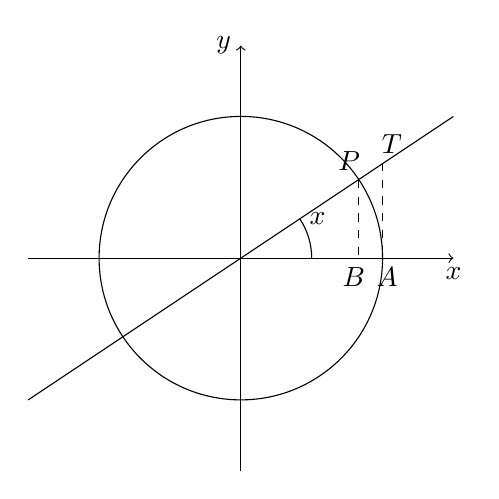
\begin{tikzpicture}[scale=1.8]
                \draw[->] (0,-1.5)--(0,1.5) node[left]{$y$};
                \draw[->] (-1.5,0)--(1.5,0) node[below]{$x$};
                \draw(0,0) circle (1);
                \draw(-1.5,-1)--(1.5,1);
                \draw(0.5,0) arc (0:33.7:0.5) node [right]{$x$};
                \draw[dashed](0.83,0.55) node [above] {$P~~$}to (0.83,0) node [below] {$B~$};
                \draw[dashed](1,0.67) node [above] {$~~T$}to (1,0) node [below] {$~A$};
            \end{tikzpicture}\\
        \caption{La situazione utilizzata per la dimostrazione}
        \label{fig:sinx}
    \end{figure}
    Per definizione si ha che \[\wideparen{PA}=x\]\[\overline{PB}=\sin x\] \[\overline{TA}=\tg x\] 
    Come è chiaramente visibile dalla Figura \ref{fig:sinx} si ha che \[\sin x < x < \tg x\] da cui \[\frac{\sin x}{\sin x}<\frac{ x}{\sin x}<\frac{\tg x}{\sin x}\] \[1<\frac{ x}{\sin x}<\frac{\tg x}{\sin x}\] \[1<\frac{\sin x}{x}<\cos x\]
    Si calcolano ora i limiti delle funzioni che limitano quella studiata
    \[\lim_{x \to 0^+}1=1 ~~~~~ \lim_{x \to 0^+}\cos x=1\]
    da cui per il teorema del confronto \[\lim_{x\to 0^+} \frac{\sin x}{x}=1\] Siccome la funzione è pari vale anche per $x\to0^-$
\end{proof}
\textbf{Osservazioni:}
\begin{itemize}
    \item vale il reciproco: $\lim_{x\to 0}\frac{x}{\sin x}=1$
    \item vale la generalizzazione: $\lim_{f(x)\to 0}\frac{\sin f(x)}{f(x)}=1$
    \item asintotico associato: $\sin x \sim x ~~~~\textnormal{in } I(0)$
\end{itemize}
\item {$\lim_{x\to 0}\frac{\tg x}{x}=1$}~
\\\begin{proof}
    Per definizione $\tg x=\frac{\sin x}{\cos x}$, quindi \[\lim_{x\to 0} \frac{\tg x}{x}=\left[\frac{0}{0}\right]\overset{FI}{=}\lim_{x\to 0} \frac{\sin x}{x \cos x}\underset{LN}{=}\lim_{x\to 0} \frac{1}{\cos x}=1\]
\end{proof}
\textbf{Osservazioni:}
\begin{itemize}
    \item vale il reciproco: $\lim_{x\to 0}\frac{x}{\tg x}=1$
    \item vale la generalizzazione: $\lim_{f(x)\to 0}\frac{\tg f(x)}{f(x)}=1$
    \item asintotico associato: $\tg x \sim x ~~~~\textnormal{in } I(0)$
\end{itemize}

\item {$\lim_{x\to 0}\frac{1-\cos x}{x}=0$}
\begin{proof}
\[\lim_{x\to 0} \frac{1-\cos x}{x}=\left[\frac{0}{0}\right]\overset{FI}{=}\lim_{x\to 0}\frac{(1-\cos x)(1+\cos x)}{x(1+\cos x)}=\lim_{x\to 0}\frac{1-\cos^2 x}{x(1+\cos x)}=\]Per la prima relazione fondamentale della goniometria\[=\lim_{x\to 0}\frac{\sin^2 x}{x(1+\cos x)}\underset{LN}{=}\lim_{x\to 0}\frac{\sin x}{1+\cos x}=\left[\frac{0}{2}\right]=0\]
\end{proof}
\textbf{Osservazioni:}
\begin{itemize}
    \item NON vale il reciproco
    \item vale la generalizzazione: $\lim_{f(x)\to 0}\frac{1-\cos f(x)}{f(x)}=1$
\end{itemize}

\item {$\lim_{x\to 0}\frac{1-\cos x}{x^2}=\frac{1}{2}$}
\begin{proof}
\[\lim_{x\to 0} \frac{1-\cos x}{x^2}=\left[\frac{0}{0}\right]\overset{FI}{=}\lim_{x\to 0}\frac{(1-\cos x)(1+\cos x)}{x^2(1+\cos x)}=\lim_{x\to 0}\frac{1-\cos^2 x}{x^2(1+\cos x)}=\]Per la prima relazione fondamentale della goniometria\[=\lim_{x\to 0}\frac{\sin^2 x}{x^2(1+\cos x)}\underset{LN}{=}\lim_{x\to 0}\frac{1}{1+\cos x}=\frac{1}{2}\]
\end{proof}
\textbf{Osservazioni:}
\begin{itemize}
    \item vale il reciproco: $\lim_{x\to 0}\frac{x^2}{1-\cos x}=1$
    \item vale la generalizzazione: $\lim_{f(x)\to 0}\frac{1- \cos f(x)}{[f(x)]^2}=1$
    \item asintotico associato: $\cos x \sim 1 - x^2 ~~~~\textnormal{in } I(0)$
\end{itemize}

\item {$\lim_{x\to +\infty}\left(1+\frac{1}{x}\right)^{x} = e$}~\vspace{10pt}\\
\textbf{Osservazioni:}
\begin{itemize}
    \item NON vale il reciproco
    \item vale la generalizzazione
\end{itemize}

\paragraph{$\lim_{x\to +\infty}\left(1+\frac{k}{x}\right)^{x} = e^k$}~\vspace{10pt}\\
\textbf{Osservazioni:}
\begin{itemize}
    \item NON vale il reciproco
    \item vale la generalizzazione
\end{itemize}

\paragraph{$\lim_{x\to 0^+}\left(1+kx\right)^{\frac{1}{x}}  e^k$}~\vspace{10pt}\\
\textbf{Osservazioni:}
\begin{itemize}
    \item NON vale il reciproco
    \item vale la generalizzazione
\end{itemize}

\item {$\lim_{x\to 0}\frac{\log_a(1+x)}{x}=\log_ae=\frac{1}{\ln a}~~~~~~~~\textnormal{con }a>0$}
\begin{proof}
\[\lim_{x\to 0}\frac{\log_a(1+x)}{x}=\left[\frac{0}{0}\right]\overset{FI}{=}\lim_{x\to 0}\frac{1}{x}\log_a(1+x)=\lim_{x\to 0}\log_a(1+x)^\frac{1}{x}=\log_ae=\frac{\ln e}{\ln a}=\frac{1}{\ln a}\]
\end{proof}
Particolarizzazione: $\lim_{x\to0}\frac{\ln(1+x)}{x}=1$~\vspace{10pt}\\
\textbf{Osservazioni:}
\begin{itemize}
    \item vale il reciproco
    \item vale la generalizzazione
    \item asintotico associato: $\ln x \sim x - 1 ~~~~\textnormal{in } I(0)$
\end{itemize}

\item {$\lim_{x\to 0}\frac{a^x-1}{x}=\ln a~~~~~~~~\textnormal{con }a>0$}
\begin{proof}
Pongo $t=a^x-1$, quindi $e^x=t+1$ e di conseguenza $x=\log_a (t+1)$. Inoltre, se $x\to 0$, $t\to 0$.
\[\lim_{x\to 0}\frac{a^x-1}{x}=\lim_{t\to 0}\frac{t}{\log_a (t+1)}=\ln a\]
\end{proof}
Particolarizzazione: $\lim_{x\to 0}\frac{e^x-1}{x}=1$~\vspace{10pt}\\
\textbf{Osservazioni:}
\begin{itemize}
    \item vale il reciproco
    \item vale la generalizzazione
    \item asintotico associato: $e^x \sim x + 1 ~~~~\textnormal{in } I(0)$
\end{itemize}

\item {$\lim_{x\to 0}\frac{(1+x)^k-1}{x}=k$}~\vspace{10pt}\\
\textbf{Osservazioni:}
\begin{itemize}
    \item vale il reciproco
    \item vale la generalizzazione
    \item asintotico associato: $(1+x)^k \sim 1+kx ~~~~\textnormal{in } I(0)$
\end{itemize}
\end{itemize}
\section{Limiti e parametri}
\begin{ex}
    [
        Trovare per quale valore di $a$ la funzione 
        \[f(x)=\begin{cases}
            2x^2-ax+1 &  x\leq -1\\
            \frac{ax-1}{x+2} &  x>1
        \end{cases}\]
        è continua in $x_0=-1$.
    ]
    Ricordando la definizione di continuità, dobbiamo determinare $a$ tale che
    \[\lim_{x\to x_0^+}f(x)=\lim_{x\to x_0^-}f(x)=f(x_0).\]
    Calcoliamo quindi 
    \[\begin{aligned}
        &\lim_{x\to-1^-}2x^2-ax+1= 3+a\qquad
        &\lim_{x\to-1^-}\frac{ax-1}{x+2}= -a-1\\
    \end{aligned}\]
    \[f(-1)= 2(-1)^2-a(-1)+1= 3+a\]
    Imponiamo l'uguaglianza
    \[\begin{cases}
        3+a=3+a\\
        -a-1=3+a
    \end{cases}\quad-a-1=3+a\qquad 2a=-4\qquad \boxed{a=-2}\]
\end{ex}
\begin{ex}
    [Determinare il valore di \[\lim_{x\to +\infty}\frac{(x-2)^n}{x^2+3x-10}\] al variare di $n\in \N$.]
    \begin{itemize}
        \item se $n=0$, \quad $\lim_{x\to +\infty}\frac{1}{x^2+3x-10}= \left[ \frac{1}{+\infty}\right]=0^+$
        \item se $n=1$, \quad $\lim_{x\to +\infty}\frac{\cancel{x-2}}{\cancel{(x-2)}(x+5)}= \left[ \frac{1}{+\infty}\right]=0^+$
        \item se $n=2$, \quad $\lim_{x\to +\infty}\frac{(x-2)^{\cancel{2}}}{\cancel{(x-2)}(x+5)}= \left[ \frac{\infty}{\infty}\right]\overset{FI}{=}1$
        \item se $n>2$, \quad $\lim_{x\to +\infty}\frac{(x-2)^{\cancel{n}^{n-1}}}{\cancel{(x-2)}(x+5)}= \left[ \frac{\infty}{\infty}\right]\overset{FI}{=}+\infty$
    \end{itemize}
\end{ex}
\section{Continuità e discontinuità}
\subsection{Discontinuità di prima specie o di salto}
\begin{boxdef}[Punti di discontinuità di prima specie]
    Un punto $x_0$ è un punto di discontinuità di prima specie per la funzione $f(x)$ quando, per $x\to x_0$ il limite destro e il limite sinistro sono finiti ma diversi.
    \[\lim_{x\to x_0^-}f(x)=l_1\qquad \lim_{x\to x_0^+}f(x)=l_2\qquad l_1\neq l_2.\]
    La differenza $|l_1-l_2|$ è detta salto
\end{boxdef}
\begin{figure}[h]
    \centering
    \begin{tikzpicture}[line cap=round,line join=round,>=triangle 45,x=1.0cm,y=1.0cm]
    \begin{axis}[
    x=1.0cm,y=1.0cm,
    axis lines=middle,
    ymajorgrids=true,
    xmajorgrids=true,
    xmin=-4.5,
    xmax=5.5,
    ymin=-2.5,
    ymax=4.5,
    xtick={-4.0,-3.0,...,5.0},
    ytick={-2.0,-1.0,...,4.0},]
    \clip(-4.5,-2.5) rectangle (5.5,4.5);
    \draw[line width=2.pt,color=red,smooth,samples=100,domain=-4.5:1.500000000000001] plot(\x,{1/50*((\x)+0*sqrt(1.5-(\x))+4)*((\x)+0*sqrt(1.5-(\x)))*((\x)+0*sqrt(1.5-(\x))-3)*((\x)+0*sqrt(1.5-(\x))-6)});
    \draw[line width=2.pt,color=red,smooth,samples=100,domain=1.500000000000001:5.5] plot(\x,{1/50*((\x)+0*sqrt(-1.5+(\x))+4)*((\x)+0*sqrt(-1.5+(\x)))*((\x)+0*sqrt(-1.5+(\x))-3)*((\x)+0*sqrt(-1.5+(\x))-6)+1.5});
    \draw [line width=2.pt,color=red, fill=white] (1.5,1.11375) circle (0.1cm);
    \draw [line width=2.pt,color=red, fill=white] (1.5,2.61375) circle (0.1cm);
    \draw (1.45,1.85) node[anchor=east, fill=white] {$salto~\Bigg\{ $};

    \draw[line width=1.pt,dash pattern=on 4pt off 4pt,smooth,samples=100,domain=6.38378239159465E-16:1.4999985000000036] plot(\x,{1/50*(1.5+4)*1.5*(1.5-3)*(1.5-6)+0*sqrt(-((\x)*((\x)-1.5)))});
    \draw[line width=1.pt,dash pattern=on 4pt off 4pt,smooth,samples=100,domain=6.38378239159465E-16:1.4999985000000036] plot(\x,{1/50*(1.5+4)*1.5*(1.5-3)*(1.5-6)+0*sqrt(-((\x)*((\x)-1.5)))+1.5});
    \draw [line width=1.pt,dash pattern=on 4pt off 4pt] (1.5,2.61375)-- (1.5,-0.02);

    \draw (1.34,0) node[anchor=north west] {$x_0$};
    \draw (-0.44,2.9) node[anchor=north west] {$l_2$};
    \draw (-0.44,1.55) node[anchor=north west] {$l_1$};

    \end{axis}
    \end{tikzpicture}
    \caption{Discontinuità di prima specie}
\end{figure}
\subsection{Discontinuità di seconda specie}
\begin{boxdef}[Punto di discontinuità di seconda specie]
    Un punto $x_0$ si dice punto di discontinnuità di seconda specie per la funzione $f(x)$ quando, per $x\to x_0$, almeno uno dei due limiti, destro o sinistro, di $f(x)$ è finito o infinito. 
\end{boxdef}
\begin{figure}[h]
    \centering
    \begin{subfigure}{0.49\textwidth}
        \centering
        \begin{tikzpicture}[scale=0.7,line cap=round,line join=round,>=triangle 45,x=1.0cm,y=1.0cm]
        \begin{axis}[
        x=1.0cm,y=1.0cm,
        axis lines=middle,
        ymajorgrids=true,
        xmajorgrids=true,
        xmin=-3.5,
        xmax=6.5,
        ymin=-2.5,
        ymax=4.5,
        xtick={-3.0,-2.0,...,6.0},
        ytick={-2.0,-1.0,...,4.0},]
        \clip(-3.5,-2.5) rectangle (6.5,4.5);
        \draw[line width=2.pt,color=red,smooth,samples=100,domain=-3.5:1.9] plot(\x,{1/(2*((\x)-2))+1});
        \draw[line width=2.pt,color=red,smooth,samples=100,domain=2.1:6.5] plot(\x,{\x-1});
        \draw [line width=2.pt,color=red, fill=red] (2,1) circle (0.1cm);
        \draw [line width=1.pt,dash pattern=on 4pt off 4pt] (2.,-2.5) -- (2.,4.5);
        \draw (2.06,0.1) node[anchor=south west] {$x_0$};
        \end{axis}
        \end{tikzpicture}
        \caption{$\lim_{x\to x_0^-}f(x)=-\infty$}
    \end{subfigure}
    \begin{subfigure}{0.49\textwidth}
        \centering
        \begin{tikzpicture}[scale=0.7,line cap=round,line join=round,>=triangle 45,x=1.0cm,y=1.0cm]
        \begin{axis}[
        x=1.0cm,y=1.0cm,
        axis lines=middle,
        ymajorgrids=true,
        xmajorgrids=true,
        xmin=-3.5,
        xmax=6.5,
        ymin=-2.5,
        ymax=4.5,
        xtick={-3.0,-2.0,...,6.0},
        ytick={-2.0,-1.0,...,4.0},]
        \clip(-3.5,-2.5) rectangle (6.5,4.5);
        \draw[line width=2.pt,color=red,smooth,samples=1000,domain=-3.5:1.99] plot(\x,{2*sin((10/((\x)-2))*180/pi)});
        \draw[line width=2.pt,color=red,smooth,samples=100,domain=2.1:6.5] plot(\x,{\x-1});
        \draw [line width=2.pt,color=red, fill=red] (2,1) circle (0.1cm);
        \draw [line width=1.pt,dash pattern=on 4pt off 4pt] (2.,-2.5) -- (2.,4.5);
        \draw (2.06,0.1) node[anchor=south west] {$x_0$};
        \end{axis}
        \end{tikzpicture}
        \caption{$\lim_{x\to x_0^-}f(x)=\nexists$}
    \end{subfigure}
    \caption{Discontinuità di seconda specie}
\end{figure}

\subsection{Discontinuità di terza specie o eliminabili}
\begin{boxdef}[Punto di discontinuità di terza specie]
    Un punto $x_0$ si dice punto di discontinnuità di terza specie per la funzione $f(x)$ quando esiste ed è finito il limite per $x\to x_0$ e $f(x)$ non è definita o assume un valore diverso da quello del limite:
    \[x_0\notin \dom f~~~~~\lor ~~~~~ f(x_0)\neq l\] 
\end{boxdef}
\begin{figure}[h]
    \centering
    \begin{subfigure}{0.49\textwidth}
        \centering
        \begin{tikzpicture}[line cap=round,line join=round,>=triangle 45,x=1.0cm,y=1.0cm]
            \begin{axis}[
            x=1.0cm,y=1.0cm,
            axis lines=middle,
            ymajorgrids=true,
            xmajorgrids=true,
            xmin=-2.5,
            xmax=4.5,
            ymin=-2.5,
            ymax=2.5,
            xtick={-2.0,-1.0,...,4.0},
            ytick={-2.0,-1.0,...,2.0},]
            \clip(-2.5,-2.5) rectangle (4.5,2.5);
            \draw[line width=2.pt,color=red,smooth,samples=100,domain=-2.5:4.5] plot(\x,{1/50*((\x)+4)*(\x)*((\x)-3)*((\x)-6)});
            \draw [line width=2.pt,color=red, fill=white] (1.5,1.11375) circle (0.1cm);
            \draw[line width=1.pt,dash pattern=on 3pt off 3pt,smooth,samples=100,domain=1.0000000001885603E-6:1.499999166667005] plot(\x,{1/50*(1.5+4)*1.5*(1.5-3)*(1.5-6)+0*sqrt(-((\x)*((\x)-1.5)))});
            \draw (1.5,0) node[anchor=north] {$x_0$};
            \draw (-0.3801983806373771,1.5) node[anchor=north west] {$l$};
            \draw [line width=1.pt,dash pattern=on 3pt off 3pt] (1.5,1.11375)-- (1.5,-0.02);
            \end{axis}
            \end{tikzpicture}
        \caption{}
    \end{subfigure}
    \begin{subfigure}{0.49\textwidth}
        \centering
        \begin{tikzpicture}[line cap=round,line join=round,>=triangle 45,x=1.0cm,y=1.0cm]
            \begin{axis}[
            x=1.0cm,y=1.0cm,
            axis lines=middle,
            ymajorgrids=true,
            xmajorgrids=true,
            xmin=-2.5,
            xmax=4.5,
            ymin=-2.5,
            ymax=2.5,
            xtick={-2.0,-1.0,...,4.0},
            ytick={-2.0,-1.0,...,2.0},]
            \clip(-2.5,-2.5) rectangle (4.5,2.5);
            \draw[line width=2.pt,color=red,smooth,samples=100,domain=-2.5:4.5] plot(\x,{1/50*((\x)+4)*(\x)*((\x)-3)*((\x)-6)});
            \draw [line width=2.pt,color=red, fill=white] (1.5,1.11375) circle (0.1cm);
            \draw[line width=1.pt,dash pattern=on 3pt off 3pt,smooth,samples=100,domain=1.0000000001885603E-6:1.499999166667005] plot(\x,{1/50*(1.5+4)*1.5*(1.5-3)*(1.5-6)+0*sqrt(-((\x)*((\x)-1.5)))});
            \draw (1.5,0) node[anchor=north] {$x_0$};
            \draw (-0.3801983806373771,1.5) node[anchor=north west] {$l$};
            \draw [line width=2.pt,color=red,fill=red,fill opacity=1.0] (1.5,1.8) circle (0.1cm);
            \draw [line width=1.pt,dash pattern=on 3pt off 3pt] (1.5,1.8)-- (1.5,-0.02);
            \draw[line width=1.pt,dash pattern=on 3pt off 3pt,smooth,samples=100,domain=1.0000000001885603E-6:1.499999166667005] plot(\x,{1.8+0*sqrt(-((\x)*((\x)-1.5)))});
            \draw (-1,1.95) node[anchor=north west] {$f(x_0)$};

            \end{axis}
            \end{tikzpicture}
        \caption{Discontinuità di terza specie}
    \end{subfigure}
    \caption{}
\end{figure}

    \begin{table}[h]
        \centering
        \begin{tabular}{|m{0.3\textwidth}|m{0.6\textwidth}|}
            \hline
            \multicolumn{2}{|m{0.9\textwidth}|}{\textbf{Discontinuità: tipologie e condizioni}}\\
            \hline
            Prima specie &  \[\lim_{x\rightarrow x_0^-}f(x)=l_1~~~~\lim_{x\rightarrow x_0^+}f(x)=l_2\] \[l_1\neq l_2~~~~salto=|l_1-l_2|\]\\ \hline
            Seconda specie &  \[\lim_{x\rightarrow x_0^\pm}f(x)=\infty ~~~~\lor~~~~ \lim_{x\rightarrow x_0^\pm}f(x)=\nexists\] \\\hline
            Terza specie & \[\lim_{x\rightarrow x_0^-}f(x)=\lim_{x\rightarrow x_0^+}f(x)=l\]\[f(x_0)\neq l ~~~~ \lor ~~~~ f(x_0)=\nexists\]\\ \hline
        \end{tabular}
    \end{table}
\subsection{Continuità e funzioni inverse}
    \subsubsection{Continuità della funzione inversa}
        \begin{shadedTheorem}[Continuità della funzione inversa]
            Se $y=f(x)$ è una funzione biiettiva e continua in un intervallo $D$, allora la funzione inversa $f^{-1}$ è continua nel codominio di $f$.
        \end{shadedTheorem}
        \begin{tabular}{m{0.45\textwidth}m{0.45\textwidth}}
            \textit{Ipotesi} & \textit{Tesi}  \\
            $f:D\to C$ biiettiva e continua in D & $f^{-1}:C\to D$ continua in C 
        \end{tabular}
        
    \subsubsection{Condizione di invertibilità per funzioni continue}
        \begin{shadedTheorem}[Invertibilità di funzioni continue]
            Sia $I$ un intervallo (limitato o illimitato) e $f:I\rightarrow \R$ una funzione continua in $I$. Allora essa è invertibile se e solo se è strettamente monotona.
        \end{shadedTheorem}
        \begin{tabular}{m{0.45\textwidth}m{0.45\textwidth}}
            \textit{Ipotesi} & \textit{Tesi}  \\
            $f:I\to \R$ continua e strettamente monotona in $I$ & $f$ è invertibile 
        \end{tabular}
    
\section{Teoremi sulle funzioni continue}
    \subsection{Teorema di Weistrass}
        \begin{shadedTheorem}[Weistrass]
            Se $f$ è una funzione continua in un intervallo limitato e chiuso $[a;b]$, allora essa assume in tale intervallo il massimo assoluto e il minimo assoluto.
        \end{shadedTheorem}
        \begin{tabular}{m{0.45\textwidth}m{0.45\textwidth}}
            \textit{Ipotesi} & \textit{Tesi}  \\
            $f:[a;b]\to \R$ continua in $[a;b]$ & $\exists c,d \in [a,b] : f(c) = min\{f\} \land f(d) = max\{f\}$
        \end{tabular}
    
    \subsection{Teorema dell'esistenza degli zeri (o di Bolzano)}
        \begin{shadedTheorem}[Bolzano]
            Se $f$ è continua in un intervallo limitato e chiuso $[a;b]$ e negli estremi di tale intervallo assume valori di segno opposto, allora esiste almeno un punto $c$ interno all'intervallo in cui $f(c)=0$.
        \end{shadedTheorem}
        \begin{tabular}{m{0.45\textwidth}m{0.45\textwidth}}
            \textit{Ipotesi} & \textit{Tesi}  \\
            \begin{enumerate}
                \item $f: [a;b] \to \R$ continua in $[a;b]$
                \item $f(a) \cdot f(b)<0$
            \end{enumerate} & $\exists c \in [a;b]:f(c)=0$ 
        \end{tabular}
    
    \subsection{Teorema dei valori intermedi (o di Darboux)}
        \begin{shadedTheorem}[Darbaux]
            Se $f$ è una funzione continua in un intervallo limitato e chiuso $[a;b]$, allora essa assume almeno una volta tutti i valori compresi tra il massimo e il minimo.
        \end{shadedTheorem}
        \begin{tabular}{m{0.45\textwidth}m{0.45\textwidth}}
            \textit{Ipotesi} & \textit{Tesi}  \\
            \begin{enumerate}
                \item $f: [a;b]\to \R$ continua in $[a;b]$
                \item $m=min\{[a;b]\}$ ~~~ $M=max\{[a;b]\}$
            \end{enumerate} & $\exists x \in [a,b] : f(x)=k \forall k \in [m;M]$
        \end{tabular}


%%%%%%%%%%%%%%%%%%%%%%%%%%%%%%%%%%%%%%%%%%%%%%%%%%%%%%%%%%%%%%%%%%%%%%%%%%%%%%%%%%%%%%%%
%%%%%%%%%%%%%%%%%%%%%%%%%%%%%%%%%%%%%%%%%%%%%%%%%%%%%%%%%%%%%%%%%%%%%%%%%%%%%%%%%%%%%%%%
%%%%%%%%%%%%%%%%%%%%%%%%%%%%%%%%%%%%%%%%%%%%%%%%%%%%%%%%%%%%%%%%%%%%%%%%%%%%%%%%%%%%%%%%
%%%%%%%%%%%%%%%%%%%%%%%%%%%%%%%%%%%%%%%%%%%%%%%%%%%%%%%%%%%%%%%%%%%%%%%%%%%%%%%%%%%%%%%%
%%%%%%%%%%%%%%%%%%%%%%%%%%%%%%%%%%%%%%%%%%%%%%%%%%%%%%%%%%%%%%%%%%%%%%%%%%%%%%%%%%%%%%%%
%%%%%%%%%%%%%%%%%%%%%%%%%%%%%%%%%%%%%%%%%%%%%%%%%%%%%%%%%%%%%%%%%%%%%%%%%%%%%%%%%%%%%%%%
%%%%%%%%%%%%%%%%%%%%%%%%%%%%%%%%%%%%%%%%%%%%%%%%%%%%%%%%%%%%%%%%%%%%%%%%%%%%%%%%%%%%%%%%
%%%%%%%%%%%%%%%%%%%%%%%%%%%%%%%%%%%%%%%%%%%%%%%%%%%%%%%%%%%%%%%%%%%%%%%%%%%%%%%%%%%%%%%%
%%%%%%%%%%%%%%%%%%%%%%%%%%%%%%%%%%%%%%%%%%%%%%%%%%%%%%%%%%%%%%%%%%%%%%%%%%%%%%%%%%%%%%%%

\chapter{Derivate}

\section{Definizione}
Consideriamo una funzione ed un punto appartenente ad essa, vorremmo avere uno strumento che, localmente, ci permetta di valutare la velocità di variazione della funzione, ovvero che in ogni punto ci dica quanto cresce la funzione.
\begin{figure}[h]
    \centering
    \begin{tikzpicture}[line cap=round,line join=round,>=triangle 45,x=1.0cm,y=1.0cm]
    \begin{axis}[
    x=1.0cm,y=1.0cm,
    axis lines=middle,
    xmin=-4.5,
    xmax=7.5,
    ymin=-2.0,
    ymax=6.5,
    xtick={0},
    ytick={0},
    xlabel={$x$},
    ylabel={$y$}]
    \clip(-4.5,-2.) rectangle (7.5,6.5);
    \draw[line width=2.pt,color=blue,smooth,samples=100,domain=-4.5:7.5] plot(\x,{2.917199344467413E-4*((\x)+2)^(5.0)-0.008389635708429067*((\x)+2)^(4.0)+0.08701740981513369*((\x)+2)^(3.0)-0.21123915819511374*((\x)+2)^(2.0)-0.312589749997511*((\x)+2)+2.6234284775953713});
    \draw [line width=1.pt,dash pattern=on 3pt off 3pt] (2.,1.7133316461676853)-- (2.,0.);
    \draw [line width=1.pt,dash pattern=on 3pt off 3pt] (5.,4.690974644951268)-- (5.,0.);
    \draw [line width=1.pt,dash pattern=on 3pt off 3pt] (5.,4.690974644951268)-- (0.,4.690974644951268);
    \draw [line width=1.pt,dash pattern=on 3pt off 3pt] (2.,1.7133316461676853)-- (0.03161971351260199,1.7133316461676853);
    \draw (1.7883695460973188,0.04068717636756156) node[anchor=north west] {$x_0$};
    \draw (4.450058466939951,0.04068717636756156) node[anchor=north west] {$x_0+h$};
    \draw (-0.1,1.69) node[anchor=east] {$f(x_0)$};
    \draw (-0.1,4.69) node[anchor=east] {$f(x_0+h)$};
    \draw (3.5,-0.5) node[anchor=north] {$\underbrace{\hspace{3cm}}_{\textstyle h}$};
    \draw [line width=2.pt,color=red, -latex] (0.03161971351260199,1.7133316461676853)-- node[right] {$\Delta y$}(0.,4.690974644951268);
    \draw [line width=2.pt,color=red, -latex] (2.,0.)--node [above]{$\Delta x$} (5.,0.);
    \begin{scriptsize}
    \draw [fill=black] (2.,1.7133316461676853) circle (2.5pt);
    \draw [fill=black] (5.,4.690974644951268) circle (2.0pt);
    \end{scriptsize}
    \node [anchor=north east] at (0,0) {$O$};
    \node [anchor=north west, color=blue] at (-4.1,1.3) {$y=f(x)$};
    \end{axis}
    \end{tikzpicture}
    \caption{}
\end{figure}
Per le rette esiste uno strumento del genere, il coefficiente angolare, che è definito come 
\[m=\frac{\Delta y}{\Delta z}\]
Proviamo quindi a definire qualcosa di simile per una funzione qualsiasi:
\begin{boxdef}[Rapporto incrementale]
    Sia $f:\:]a,b[\to \R$ , $x_0\in ]a,b[$, definiamo \textbf{rapporto incrementale} di $f$ tra il punto $x_0$ e il punto $x_1=x_0+h$ (con $h\neq 0$) la grandezza :
    \[R.I.=\frac{\Delta y}{\Delta x}=\frac{f(x_1)-f(x_0)}{x_1-x_0}=\frac{f(x_0+h)-f(x_0)}{h}\]
\end{boxdef}
Tuttavia questo strumento ci da informazioni sulla crescita media della funzione nell'intervallo $[x_0,x_1]$, a noi serve qualcosa di relativo al solo punto $x_0$, per cui facciamo avvicinare $x_1$ a $x_0$, quindi otteniamo
\[\lim_{\Delta x \to 0}\frac{\Delta y}{\Delta x}=\lim_{x_1\to x_0}\frac{f(x_1)-f(x_0)}{x_1-x_0}=\lim_{h\to 0}\frac{f(x_0+h)-f(x_0)}{h}.\]
Definiamo quindi la derivata, ovvero lo strumento che ci permette di conoscere localmente la velocità di variazione di una funzione:
\begin{boxdef}[Derivata]
    Data una funzione $f:[a,b]\to\R$, $f$ il limite per $x_1\to x_0$ del rapporto incrementale tra $x_1$ e $x_0$, se esiste ed è finitl, si definisce \textbf{derivata prima della funzione}  in $x_0$
    \[f'(x_0)=\lim_{\Delta x \to 0}\frac{\Delta y}{\Delta x}=\lim_{x_1\to x_0}\frac{f(x_1)-f(x_0)}{x_1-x_0}=\lim_{h\to 0}\frac{f(x_0+h)-f(x_0)}{h}.\]
\end{boxdef}
In quanto limite, la derivata esiste solo se esistono limite destro e sinistro e sono uguali. Definiamo quindi \textbf{derivata sinistra e destra}
\[f'_-(x_0)=\lim_{h\to x_0^-}\frac{f(x_0+h)-f(x_0)}{h}\qquad \qquad f'_+(x_0)=\lim_{h\to x_0^+}\frac{f(x_0+h)-f(x_0)}{h}\]
\subsection{Problema classico}
Il concetto di derivata nasce anche per risolvere un problema classico della matematica: nota una funzione e un suo punto $P(x_0,f(x_0))$, determinare l'equazione della retta tangente alla curva in $P$. 

Per farlo, è possibile introdurre un secondo punto $Q(x_0+h, f(x_0+h))$ e calcolare la retta passante per i due punti (secante). Sappiamo che l'equazione della retta passante per due punti è data da
\[PQ:\qquad \frac{x-x_P}{x_Q-x_P}=\frac{y-y_P}{y_Q-y_P}\]
sostituendo otteniamo
\[\frac{y-f(x_0)}{f(x_0+h)-f(x_0)}=\frac{x-x_0}{x_0+h-x_0}.\]
Riconducento quindi la scrittura all'equazione della retta per un punto noto il coefficiente angolare orreniamo
\[y-f(x)=\frac{f(x_0+h)-f(x_0)}{h}(x-x_0)\]
Si ricava quindi che il rapporto incrementale è il il coefficiente angolare della retta secante $PQ$. Inoltre, la derivata prima si ricava quando avviciniamo al limite $P$ e $Q$, per cui è il coefficiente angolare della retta tangente nel punto $P$.
\subsection{Calcolo della derivata mediante definizione}
\begin{ex}[Calcolare la derivata di $y=4x-9$ mediante definizione.]
    \[\begin{aligned}y'=\lim_{h\to 0}\frac{f(x_0+h)-f(x_0)}{h}= \lim_{h\to x_0} \frac{\left[ 4(x+h)-9 \right]-\left[ 4x-9 \right]}{h}=\lim_{h\to 0}\frac{\cancel{4x}+4h-\cancel{9}-\cancel{4x}+\cancel{9}}{h}=\lim_{h\to0}\frac{4\cancel{h}}{\cancel{h}}=4\end{aligned}\]
\end{ex}
\begin{ex}[Calcolare la derivata di $y=-x^2+4x$ mediante definizione]
    \[\begin{aligned}
        y'&= \lim_{h\to 0} \frac{f(x+h)-f(x_0)}{h}= \lim_{h\to 0}\frac{-(x+h)^2+4(x+h)+x^2-4x}{h}=\\&=\frac{\cancel{-x^2}-h^2-2hx+\cancel{4x}+h+\cancel{x^2}-\cancel{4x}}{h}= \lim_{h\to 0}\frac{\cancel{h}(\cancel{-h}-2x+4)}{\cancel{h}}=-2x+4
    \end{aligned}\]
\end{ex}
\section{Derivate fondamentali}
\subsection{Funzione costante}
\begin{center}
    \begin{tabular}{m{0.45\textwidth}|m{0.45\textwidth}}
        \begin{center}
            \textbf{Funzione}
        \end{center}
        & 
        \begin{center}
            \textbf{Derivata}
        \end{center}\\
        \hline
            \[y=k\]&
            \[y'=0\]
    \end{tabular}
\end{center}
\begin{proof}
    \[y'=\lim_{h\to 0}\frac{k-k}{h}=\lim_{h\to 0}0=0\]
    N.B.: Non è una forma di indecisione perchè la funzione è già 0 prima di calcolare il limite.
\end{proof}

\subsection{Funzione identità}
\begin{center}
    \begin{tabular}{m{0.45\textwidth}|m{0.45\textwidth}}
        \begin{center}
            \textbf{Funzione}
        \end{center}
        & 
        \begin{center}
            \textbf{Derivata}
        \end{center}\\
        \hline
            \[y=x\]&
            \[y'=1\]
    \end{tabular}
\end{center}
\begin{proof}
    \[y'=\lim_{h\to 0}\frac{x+h-x}{h}=\lim_{h\to 0}\frac{h}{h}=\left[\frac{0}{0}\right]\overset{FI}{=}1\]
\end{proof}

\subsection{Funzione potenza}
\begin{center}
    \begin{tabular}{m{0.45\textwidth}|m{0.45\textwidth}}
        \begin{center}
            \textbf{Funzione}
        \end{center}
        & 
        \begin{center}
            \textbf{Derivata}
        \end{center}\\
        \hline
            \[y=x^\alpha~~~~~(\alpha \in \R)\]&
            \[y'=\alpha x ^{\alpha-1}\]
    \end{tabular}
\end{center}
\begin{proof}
    \[y'=\lim_{h\to 0}\frac{(x+h)^\alpha-x^\alpha}{h}=\left[ \frac{0}{0} \right]\overset{FI}{=}\lim_{h\to 0}\frac{\left[ x \left(1+\frac{h}{x}\right) \right]^\alpha -x^\alpha}{h}=\lim_{h\to 0}\frac{x^\alpha\left[\left(1+\frac{h}{x}\right)^\alpha -1\right] }{\frac{h}{x}}\underset{LN}=\alpha x^{\alpha-1}\]
\end{proof}
\subsubsection{Derivata della funzione radice quadrata}
Per la derivata delle funzioni potenza, si ricava la derivata della funzione radice quadrata:
\begin{center}
    \begin{tabular}{m{0.45\textwidth}|m{0.45\textwidth}}
        \begin{center}
            \textbf{Funzione}
        \end{center}
        & 
        \begin{center}
            \textbf{Derivata}
        \end{center}\\
        \hline
            \[y=\sqrt{x}=x^{\frac{1}{2}}\] &
            \[y'=\frac{1}{2\sqrt{x}} = \frac{1}{2}x ^{-\frac{1}{2}}\]
    \end{tabular}
\end{center}

\subsection{Funzione seno}
\begin{center}
    \begin{tabular}{m{0.45\textwidth}|m{0.45\textwidth}}
        \begin{center}
            \textbf{Funzione}
        \end{center}
        & 
        \begin{center}
            \textbf{Derivata}
        \end{center}\\
        \hline
            \[y=\sin x\]&
            \[y'=\cos x\]
    \end{tabular}
\end{center}
\begin{proof}
    \[\begin{aligned}y'&=\lim_{h\to 0}\frac{\sin(x+h)-\sin x}{h}=\left[ \frac{0}{0} \right]\overset{FI}{=}\lim_{h\to 0}\frac{\sin x \cos h + \cos x \sin h - \sin x}{h}=\\&=\lim_{h\to 0}\left(\sin x\,\underset{LN=0}{\boxed{\frac{\cos h-1}{h}}}+\cos x\,\underset{LN=1}{\boxed{\frac{\sin h}{h}}}\right)\underset{LN}=\cos x\end{aligned}\]
\end{proof}

\subsection{Funzione coseno}
\begin{center}
    \begin{tabular}{m{0.45\textwidth}|m{0.45\textwidth}}
        \begin{center}
            \textbf{Funzione}
        \end{center}
        & 
        \begin{center}
            \textbf{Derivata}
        \end{center}\\
        \hline
            \[y=\cos x\]&
            \[y'=- \sin x\]
    \end{tabular}
\end{center}
\begin{proof}
    \[\begin{aligned}y'&=\lim_{h\to 0}\frac{\cos(x+h)-\cos x}{h}=\left[ \frac{0}{0} \right]\overset{FI}{=}\lim_{h\to 0}\frac{\cos x \cos h - \sin x \sin h - \cos x}{h}=\\&=\lim_{h\to 0}\left(\cos x\,\underset{LN=0}{\boxed{\frac{\cos h-1}{h}}}-\sin x\,\underset{LN=1}{\boxed{\frac{\sin h}{h}}}\right)\underset{LN}=-\sin x\end{aligned}\]
\end{proof}

\subsection{Funzione esponenziale}
\begin{center}
    \begin{tabular}{m{0.45\textwidth}|m{0.45\textwidth}}
        \begin{center}
            \textbf{Funzione}
        \end{center}
        & 
        \begin{center}
            \textbf{Derivata}
        \end{center}\\
        \hline
            \[y=a^x\]&
            \[y'=a^x\ln a\] \\
            \[y=e^x\] & 
            \[y'=e^x\]
    \end{tabular}
\end{center}
\begin{proof}
    \[\begin{aligned}y'&=\lim_{h\to 0}\frac{a^{x+h}-a^x}{h}=\left[ \frac{0}{0} \right]\overset{FI}{=}\lim_{h\to 0}\frac{a^xa^h-a^x}{h}=\lim_{h\to 0}a^x\,\underset{LN=\ln a}{\boxed{\frac{a^h-1}{h}}}\underset{LN}=a^x\ln a\end{aligned}\]
\end{proof}

\subsection{Funzione logaritmo}
\begin{center}
    \begin{tabular}{m{0.45\textwidth}|m{0.45\textwidth}}
        \begin{center}
            \textbf{Funzione}
        \end{center}
        & 
        \begin{center}
            \textbf{Derivata}
        \end{center}\\
        \hline
            \[y=\log_a x\]&
            \[y'=\frac{1}{x} \log_a e\] \\
            \[y=\ln x\] & 
            \[y'=\frac{1}{x}\]
    \end{tabular}
\end{center}
\begin{proof}
    \[\begin{aligned}y'&=\lim_{h\to 0}\frac{\log_a(x+h)-\log_a x}{h}=\left[ \frac{0}{0} \right]\overset{FI}{=}\lim_{h\to 0}\frac{\log_a\left(\frac{x+h}{h}\right)}{h}=\lim_{h\to 0}\underset{LN=\log_a e}{\boxed{\frac{\log_a\left(1+\frac{x}{h}\right)}{\frac{h}{x}}}\cdot\frac{1}{x} }\underset{LN}=\frac{1}{x}\log_ae\end{aligned}\]
\end{proof}

\section{Operazioni con le derivate}
    \subsection{Linearità rispetto al prodotto}
    La derivata è lineare rispetto al prodotto per costanti, quindi possiamo \say{portare fuori} le costanti dalla derivata. In simboli ($k\in\R$):
    \[y=k\cdot f(x)\qquad \qquad y'=k\cdot f'(x).\]
    \begin{ex}[Calcolare la derivata delle seguenti funzioni: 
        \begin{tasks}(2)
            \task $f(x)=\sqrt{2}\sin x$
            \task $g(x)=3\ln x$
        \end{tasks}
        ]
        \begin{tasks}(2)
            \task $f'(x)=\sqrt{2}\cos x$
            \task $g'(x)=\frac{3}{x}$
        \end{tasks}
    \end{ex}
    \subsection{Linearità rispetto alla somma}
    La derivata è lineare rispetto alla somma, per cui la derivata della somma di due funzioni è la somma delle derivare delle funzioni stesse:
    \[y=f(x)+g(x)\qquad \qquad y'=f'(x)+g'(x).\]
    \begin{ex}[
        Calcolare la derivata delle seguenti funzioni
        \begin{tasks}(2)
            \task $y=5x^3+e^x$
            \task $y=-\frac{1}{2}x^2+x+1$
        \end{tasks}
    ]
    \begin{tasks}(2)
        \task $y=15x^2+e^x$
        \task $y=-x+1$
    \end{tasks}
    \end{ex}

    \subsection{Derivata del prodotto}
    La derivata del prodotto di due funzioni NON è il prodotto  delle derivate delle funzioni, ma si ottiene sommando la derivata della prima moltiplicata per la seconda e la derivata della seconda moltiplicata per la prima:
    \[y=f(x)g(x)\qquad\qquad y'=f'(x)g(x)+f(x)g'(x)\]
    \begin{ex}[
        Calcolare la derivata delle seguenti funzioni
        \begin{tasks}(2)
            \task $y=x^2\cdot \cos x$
            \task $y=x\cdot e^x\cdot \ln x$
        \end{tasks}
    ]
    \begin{tasks}(2)
        \task $y'=2x\cos x+ x^2\sin x$
        \task $y'=1\cdot e^x \cdot \ln x+ x\cdot e^x\cdot \ln x+ x\cdot e^x \cdot \frac{1}{x}$
    \end{tasks}
    \end{ex}

    \subsection{Derivata del rapporto}
    Analogamente, la derivata del rapporto NON è il rapporto delle derivate ma 
    \[t=\frac{f(x)}{g(x)}=\frac{f'(x)g(x)-f(x)g'(x)}{[g(x)]^2}.\]
    Da questa formula segue anche la formula della derivata del reciproco:
    \[y=\frac{1}{f(x)}\qquad \qquad y=\frac{f'(x)}{[f(x)]^2}\]
    \begin{ex}[
        Calcolare la derivata delle seguenti funzioni
        \begin{tasks}(2)
            \task $y=\frac{5+x}{2x^2}$
            \task $y=\frac{1}{2x^3+3}$
        \end{tasks}
    ]
    \begin{tasks}(2)
        \task $y=\frac{1\cdot (2x^2)-(5+x)(4x)}{2x^2}$
        \task $y=\frac{6x^2}{(2x^3+3)^2}$
    \end{tasks}
\end{ex}

\subsection{Derivata della funzione composta (chain rule)}
Per derivare una funzione composta bisogna procedere "a guscio": osservando la funzione da derivare, procedere dall'interno verso l'esterno derivando ogni strato e moltiplicando il tutto:
\[y=f(g(x))\qquad\qquad y'=f'(g(x))\cdot g'(x)\]
\begin{ex}[
    Calcolare la derivata delle seguenti funzioni
        \begin{tasks}(2)
            \task $y={[f(x)]}^{\alpha}$
            \task $y=\sin f(x)$
            \task $y=a^{f(x)}$
            \task $y=\sin(\ln(2x))$
            \task $y=\frac{\sin (2x)}{\cos (3x)}$
            \task $y=\cos(x)\cdot \ln (x^2+3x)$
        \end{tasks}
    ]
    Calcolare la derivata delle seguenti funzioni
    \begin{tasks}(2)
        \task $y'=\alpha{[f(x)]}^{\alpha-1}\cdot f'(x)$
        \task $y'=f'(x)\cdot\cos f(x)$
        \task $y'=a^{f(x)}\cdot \ln a \cdot f'(x)$
        \task $y'=\cos(\ln (2x))\cdot \frac{1}{2x}\cdot 2$
        \task $y'=\frac{[2\cos (2x)]\cdot \cos (3x)-\sin(2x)\cdot[-3\sin(3x)]}{[\cos (3x)]^2}$
    \end{tasks}
    \begin{tasks}[resume]
        \task $y'=-\sin(x)\cdot \ln (x^2+3x)+\cos(x)\cdot \frac{1}{x^2+3x}\cdot\left( 2x+3 \right)$
    \end{tasks}
\end{ex}
\section{Derivate notevoli /2}
\subsection{Funzione tangente}
\begin{center}
    \begin{tabular}{m{0.45\textwidth}|m{0.45\textwidth}}
        \begin{center}
            \textbf{Funzione}
        \end{center}
        & 
        \begin{center}
            \textbf{Derivata}
        \end{center}\\
        \hline
            \[y=\tg x\] &
            \[y'=\frac{1}{\cos^2x}=1+\tg^2x\]
    \end{tabular}
\end{center}
    \begin{proof}
        Ricordiamo che $y=\tg x =\frac{\sin x}{\cos x}$, quindi 
        \[\begin{aligned}
            y'=\frac{\cos^2 x+\sin^2 x}{\cos^2 x} &= \frac{1}{\cos^2 x}\\
                                                  &= 1+ \frac{\sin^2x}{\cos^2x }= 1+\tg^2x 
        \end{aligned}\]
    \end{proof}
\subsection{Funzione cotangente}
\begin{center}
    \begin{tabular}{m{0.45\textwidth}|m{0.45\textwidth}}
        \begin{center}
            \textbf{Funzione}
        \end{center}
        & 
        \begin{center}
            \textbf{Derivata}
        \end{center}\\
        \hline
            \[y=\cotg x\] &
            \[y'=-\frac{1}{\sin^2x}=-1-\cotg^2x\]
    \end{tabular}
\end{center}
    \begin{proof}
        Ricordiamo che $y=\cotg x =\frac{\cos x}{\sin x}$, quindi 
        \[\begin{aligned}
            y'=\frac{-\sin^2 x-\cos^2 x}{\sin^2 x} &= -\frac{1}{\sin^2 x}\\
                                                  &= -1- \frac{\cos^2x}{\sin^2x }= -1-\cotg^2x 
        \end{aligned}\]
    \end{proof}
\section{Legame tra continuità e derivabilità}
\subsection{Continuità delle funzioni derivabili}
\begin{shadedTheorem}[Continuità delle funzioni derivabili]
    Se una funzione $f(x)$ è derivabile in un punto $x_0$, allora essa è anche continua in $x_0$.
\end{shadedTheorem}
\begin{tabular}{m{0.48\textwidth}m{0.48\textwidth}}
    \textit{Ipotesi} & \textit{Tesi}  \\
    $f$ derivabile in $x_0$, $\exists \lim_{h\to 0}\frac{f(x_0+h)-f(x_0)}{h}=f'(x_0)$ & $f$ continua in $x_0$, $\lim_{x\to x_0}f(x)=f(x_0)$ 
\end{tabular}
\begin{proof}
    \[  \begingroup
        \addtolength{\jot}{1em}
        \begin{aligned}
        \text{vero} & \implies\\
        f(x_0+h)=f(x_0+h) & \implies\\
        f(x_0+h)=f(x_0+h)-f(x_0)+f(x_0)& \implies (\text{se }h\neq 0)\\
        f(x_0+h)=\frac{f(x_0+h)-f(x_0)}{h}\cdot h+f(x_0)& \implies (\text{limite})\\
        \lim_{h\to0}f(x_0+h)=\lim_{h\to0}\left[\frac{f(x_0+h)-f(x_0)}{h}\cdot h+f(x_0)\right] &  \implies (\text{separo perchè i limiti sono finiti})\\
        \lim_{h\to0}f(x_0+h)=\lim_{h\to0}\left[\frac{f(x_0+h)-f(x_0)}{h}\cdot h\right]+\lim_{h\to0}f(x_0) &  \implies (\text{separo perchè i limiti sono finiti})\\
        \lim_{h\to0}f(x_0+h)=\lim_{h\to0}\frac{f(x_0+h)-f(x_0)}{h}\cdot \lim_{h\to0} h+\lim_{h\to0}f(x_0) &  \implies (\text{calcolo i limiti})\\
        \lim_{h\to0}f(x_0+h)=f'(x_0)\cdot 0+f(x_0) &  \implies (\text{sostituisco ponendo }x=x_0+h)\\
        \lim_{x\to x_0}f(x)=f(x_0) 
    \end{aligned}
    \endgroup
    \]
\end{proof}
\begin{oss}[1]
    L'insieme delle funzioni derivabili è un sottoinsieme delle funzioni continue. Esistono funzioni continue ma non derivabili, mentre tutte le funzioni derivabili sono continue.
\end{oss}
\begin{oss}[2]
    La continuità è condizione necessaria ma non sufficiente della derivabilità, per cui una funzione per essere derivabile deve essere continua, ma non è detto che una funzione continua sia derivabile.
\end{oss}
\subsection{Studi di continuità e derivabilità}
\begin{ex}
    [Studiare continuità e derivabilità della funzione $y=\sqrt{4-|x|+3x}$ in $x_0=0$]
    Prima di tutto apriamo la scrittura sulla definizione di modulo
    \[y=\begin{cases}
        \sqrt{4-x+3x} & x\geq 0\\
        \sqrt{4+x+3x} & x < 0
    \end{cases} = \begin{cases}
        \sqrt{4+2x} & x\geq 0\\
        \sqrt{4+4x} & x < 0.
    \end{cases}\]
    Controlliamo ora i domini dei tratti
    \[\dom\sqrt{4+2x}=\{x\in \R\, |\, x\geq -2\}\]
    \[\dom\sqrt{4+4x}=\{x\in \R\, |\, x\geq -1\}\]
    e integriamo nella definizione della funzione
    \[y=\begin{cases}
        \sqrt{4+2x} & x\geq 0\\
        \sqrt{4+4x} & -1 \leq x < 0.
    \end{cases}\]
    Ora possiamo procedere con lo studio di continuità in $x_0=0$. Calcoliamo i limiti da sinistra e destra e il valore della funzione in $x_0$:
    \[
        f(0)=2 \qquad\qquad
        \lim_{x\to 0^-}\sqrt{4+4x}=2\qquad \qquad
        \lim_{x\to 0^+}\sqrt{4+2x}=2.
    \]
    Siccome sono uguali, otteniamo che la funzione è continua in $x_0=0$. Procediamo quindi con lo studio di derivabilità:
    \begin{ricorda}
        Una funzione è derivabile in un punto se la derivata destra e la derivata sinistra sono finite e uguali.
    \end{ricorda}
    Per ora sappiamo calcolare derivata destra e sinistra solo mediante definizione. A breve acquisiremo uno strumento che ci permetterà di calcolarle più agevolmente.
    \[f'_-(x)=\lim_{h\to0^-}\frac{f(0+h)-f(0)}{h}=\lim_{h\to0}\frac{\sqrt{4+4h}-2}{h}=\left[ \frac{0}{0} \right]\overset{FI}{=}\lim_{h\to0}\frac{\cancel{4}+4\cancel{h}-\cancel{4}}{\cancel{h}\left( \sqrt{4+4h}+2 \right)}=1\]
    \[f'_-(x)=\lim_{h\to0^-}\frac{f(0+h)-f(0)}{h}=\lim_{h\to0}\frac{\sqrt{4+2h}-2}{h}=\left[ \frac{0}{0} \right]\overset{FI}{=}\lim_{h\to0}\frac{\cancel{4}+2\cancel{h}-\cancel{4}}{\cancel{h}\left( \sqrt{4+2h}+2 \right)}=\frac{1}{2}.\]
    Di conseguenza, siccome derivata destra e sinistra sono diverse, la funzione non è derivabile in $x_0=0$.
\end{ex}
\section{Punti di non derivabilità}
Quando una funzione in un punto $x_0$ è continua ma non derivabile, possiamo classificare il tipo di punto di non derivabilità in base alla derivata destre e sinistra.
\subsection{Punto angoloso}
Quando la derivata sinistra e la derivata destra in un punto $x_0$ sono finite e diverse oppure una è infinita e l'altra finita, la funzione presenta un punto angoloso:
\begin{figure}[h]
    \centering
    \begin{subfigure}{0.49\textwidth}
        \centering
        \begin{tikzpicture}[line cap=round,line join=round,>=triangle 45,x=1.0cm,y=1.0cm]
            \begin{axis}[
            x=1.0cm,y=1.0cm,
            axis lines=middle,
            xmin=-1.0,
            xmax=4.9,
            ymin=-1.0,
            ymax=4.5,
            xtick={0.0},
            ytick={0.0},]
            \draw [samples=50,color=red,rotate around={0.:(2.,1.)},xshift=2.cm,yshift=1.cm,line width=2.pt,domain=-8.0:-1)] plot (\x,{(\x)^2/2/2.0});
            \draw [samples=50,color=red,rotate around={-180.:(2.,1.5)},xshift=2.cm,yshift=1.5cm,line width=2.pt,domain=-8.0:1.0)] plot (\x,{(\x)^2/2/2.0});
            %\draw[line width=2.pt,color=red,smooth,samples=100,domain=1.0000057000000064:6.7] plot(\x,{2*sqrt((\x)-1)+1/4*(1-2)^(2)+1});
            \draw [line width=1pt,dash pattern=on 4pt off 4pt] (1.,0.)node[below]{$x_0$} -- (1.,6.5);
            \draw [line width=1.pt,dash pattern=on 4pt off 4pt,domain=1.0:6.7] plot(\x,{(--1.059--0.706*\x)/1.412});
            \draw [line width=1.pt,dash pattern=on 4pt off 4pt,domain=-1.0:1.0] plot(\x,{(-2.933--0.838*\x)/-1.676});
            %\draw [line width=1.pt,dash pattern=on 4pt off 4pt,domain=1.0878040397002193:6.7] plot(\x,{(-1.0948156748611662--2.0207040111538945*\x)/0.5987698888599833});
            %\draw [line width=1.pt,dash pattern=on 4pt off 4pt,domain=1.2810852814081708:6.7] plot(\x,{(-0.07803990588031695--1.3887027814931505*\x)/0.7362551707876179});
            %\draw [line width=1.pt,dash pattern=on 4pt off 4pt,domain=1.0222607361887122:6.7] plot(\x,{(-4.219803377984541--5.33315991748734*\x)/0.7957091788219195});
            %\draw[red,-latex,line width=1.pt] (2.25,3.7) arc (55:85:2.5);
            %\draw [color=red](1.5,3.9) node[anchor=north] {$+\infty$};
            \end{axis}
            \end{tikzpicture}

        \caption{}
    \end{subfigure}
    \begin{subfigure}{0.49\textwidth}
        \centering
        \begin{tikzpicture}[line cap=round,line join=round,>=triangle 45,x=1.0cm,y=1.0cm]
            \begin{axis}[
            x=1.0cm,y=1.0cm,
            axis lines=middle,
            xmin=-1.0,
            xmax=4.5,
            ymin=-1.0,
            ymax=4.5,
            xtick={0},
            ytick={0},]
            \draw [samples=50, color=red, rotate around={0.:(2.,1.)},xshift=2.cm,yshift=1.cm,line width=2.pt,domain=-8.0:-1.0)] plot (\x,{(\x)^2/2/2.0});
            %\draw [samples=50,rotate around={-180.:(2.,1.5)},xshift=2.cm,yshift=1.5cm,line width=2.pt,domain=-8.0:8.0)] plot (\x,{(\x)^2/2/2.0});
            \draw[line width=2.pt,color=red,smooth,samples=100,domain=1.0000057000000064:6.7] plot(\x,{2*sqrt((\x)-1)+1/4*(1-2)^(2)+1});
            \draw [line width=1pt,dash pattern=on 4pt off 4pt] (1.,0.)node[below]{$x_0$} -- (1.,6.5);
            %\draw [line width=1.pt,dash pattern=on 4pt off 4pt,domain=1.0:6.7] plot(\x,{(--1.059--0.706*\x)/1.412});
            \draw [line width=1.pt,dash pattern=on 4pt off 4pt,domain=-1.0:1.0] plot(\x,{(-2.933--0.838*\x)/-1.676});
            \draw [line width=1.pt,dash pattern=on 4pt off 4pt,domain=1.0878040397002193:6.7] plot(\x,{(-1.0948156748611662--2.0207040111538945*\x)/0.5987698888599833});
            \draw [line width=1.pt,dash pattern=on 4pt off 4pt,domain=1.2810852814081708:6.7] plot(\x,{(-0.07803990588031695--1.3887027814931505*\x)/0.7362551707876179});
            \draw [line width=1.pt,dash pattern=on 4pt off 4pt,domain=1.0222607361887122:6.7] plot(\x,{(-4.219803377984541--5.33315991748734*\x)/0.7957091788219195});
            \draw[red,-latex,line width=1.pt] (2.25,3.7) arc (55:85:2.5);
            \draw [color=red](1.5,3.9) node[anchor=north] {$+\infty$};
            \end{axis}
            \end{tikzpicture}
        \caption{}
    \end{subfigure}
    \caption{Punti angolosi}
\end{figure}
\subsection{Cuspide}
Quando la derivata destra e la derivata sinistra in un punto $x_0$ sono infinite e diverse (una $+\infty$ e l'altra $-\infty$), la funzione presenta una cuspide:
\begin{figure}[h]
    \centering
    \begin{subfigure}{0.49\textwidth}
        \centering
        \begin{tikzpicture}[scale=1.2,line cap=round,line join=round,>=triangle 45,x=1.0cm,y=1.0cm]
            \begin{axis}[
            x=1.0cm,y=1.0cm,
            axis lines=middle,
            xmin=-1.0,
            xmax=3.0,
            ymin=-0.5,
            ymax=3.0,
            xtick={0},
            ytick={0},]
            \clip(-1.,-0.5) rectangle (3.,3.);
            \draw [line width=0.7pt,dash pattern=on 2pt off 2pt] (1.,0.)node[below]{$x_0$} -- (1.,3.);

            % NE
            \draw[line width=1.7pt,color=red,smooth,samples=100,domain=1.0:3.0] plot(\x,{sqrt((\x)-1)+1/4*(1-2)^(2)+1});
            \draw [line width=0.7pt,dash pattern=on 2pt off 2pt,domain=1.0878040397002193:3.0] plot(\x,{(-0.1985714042574651--1.1585107377700068*\x)/0.6865739285602026});
            \draw [line width=0.7pt,dash pattern=on 2pt off 2pt,domain=1.2810852814081708:3.0] plot(\x,{(--0.5819209095818256--0.9594387732302438*\x)/1.017340452195789});
            \draw [line width=0.7pt,dash pattern=on 2pt off 2pt,domain=1.0222607361887122:3.0] plot(\x,{(-1.6576970386590935--2.741180119917611*\x)/0.8179699150106317});
            \draw[red,latex-,line width=0.7pt] (1.1,2.6) arc (85:45:1);
            \node [red] at(1.6,2.8) {$+\infty$};
            
            % NO
            \draw[line width=1.7pt,color=red,smooth,samples=100,domain=-1.0:1.0] plot(\x,{sqrt(-1.0*((\x)-2.0)-1)+1/4*(1-2)^(2)+1});
            \draw [line width=0.7pt,dash pattern=on 2pt off 2pt,domain=-1.0:0.9777392638112881] plot(\x,{(-3.824663201176129--2.741180119917611*\x)/-0.8179699150106313});
            \draw [line width=0.7pt,dash pattern=on 2pt off 2pt,domain=-1.0:0.9121959602997809] plot(\x,{(-2.118450071282548--1.1585107377700068*\x)/-0.6865739285602025});
            \draw [line width=0.7pt,dash pattern=on 2pt off 2pt,domain=-1.0:0.7189147185918294] plot(\x,{(-2.500798456042313--0.9594387732302438*\x)/-1.0173404521957887});
            \draw[red,latex-,line width=0.7pt] (0.9,2.6) arc (95:135:1);
            \node [red] at(0.4,2.8) {$-\infty$};
            
            \end{axis}
            \end{tikzpicture}
        \caption{}
    \end{subfigure}
    \begin{subfigure}{0.49\textwidth}
        \centering
        \begin{tikzpicture}[scale=1.2,line cap=round,line join=round,>=triangle 45,x=1.0cm,y=1.0cm]
            \begin{axis}[
            x=1.0cm,y=1.0cm,
            axis lines=middle,
            xmin=-1.0,
            xmax=3.0,
            ymin=-0.5,
            ymax=3.0,
            xtick={0},
            ytick={0},]
            \clip(-1.,-0.5) rectangle (3.,3.);
            \draw [line width=0.7pt,dash pattern=on 2pt off 2pt] (1.,0.)node[below]{$x_0$} -- (1.,3.);

            % SO
            \draw[line width=1.7pt,color=red,smooth,samples=100,domain=-1.0:1.0] plot(\x,{(sqrt(-1.0*((\x)-2.0)-1)+1/4*(1-2)^(2)+1)*(-1.0)+2.5});
            \draw [line width=0.7pt,dash pattern=on 2pt off 2pt,domain=-1.0:0.7189147185918292] plot(\x,{(-0.04255267444715913-0.9594387732302438*\x)/-1.017340452195789});
            \draw [line width=0.7pt,dash pattern=on 2pt off 2pt,domain=-1.0:0.9121959602997807] plot(\x,{(--0.4020152498820416-1.1585107377700068*\x)/-0.6865739285602026});
            \draw [line width=0.7pt,dash pattern=on 2pt off 2pt,domain=-1.0:0.9777392638112878] plot(\x,{(--1.7797384136495498-2.741180119917611*\x)/-0.8179699150106317});
            \draw[red,latex-,line width=0.7pt] (0.9,-0.1) arc (265:225:1);
            \node [red] at(0.4,-0.3) {$+\infty$};
            
            % SE
            \draw[line width=1.7pt,color=red,smooth,samples=100,domain=1.0:3.0] plot(\x,{(sqrt((\x)-1)+1/4*(1-2)^(2)+1)*(-1.0)+2.5});
            \draw [line width=0.7pt,dash pattern=on 2pt off 2pt,domain=1.0878040397002193:3.0] plot(\x,{(--1.9150062256579723-1.1585107377700066*\x)/0.686573928560203});
            \draw [line width=0.7pt,dash pattern=on 2pt off 2pt,domain=1.281085281408171:3.0] plot(\x,{(--1.9614302209076473-0.9594387732302435*\x)/1.0173404521957892});
            \draw [line width=0.7pt,dash pattern=on 2pt off 2pt,domain=1.0222607361887122:3.0] plot(\x,{(--3.7026218261856734-2.741180119917611*\x)/0.8179699150106323});
            \draw[red,latex-,line width=0.7pt] (1.1,-0.1) arc(275:315:1);
            \node [red] at(1.6,-0.3) {$-\infty$};
            \end{axis}
            \end{tikzpicture}
        \caption{}
    \end{subfigure}
    \caption{Punti angolosi}
\end{figure}
\subsection{Flesso a tangente verticale}
Quando la derivata destra e la derivata sinistra in un punto $x_0$ sono infinite e uguali (entrambe $+\infty$ o entrambe $-\infty$), la funzione presenta un flesso a tangente verticale:
\begin{figure}[h]
    \centering
    \begin{subfigure}{0.49\textwidth}
        \centering
        \begin{tikzpicture}[scale=1.2,line cap=round,line join=round,>=triangle 45,x=1.0cm,y=1.0cm]
            \begin{axis}[
            x=1.0cm,y=1.0cm,
            axis lines=middle,
            xmin=-1.0,
            xmax=3.0,
            ymin=-0.5,
            ymax=3.0,
            xtick={0},
            ytick={0},]
            \clip(-1.,-0.5) rectangle (3.,3.);
            \draw [line width=0.7pt,dash pattern=on 2pt off 2pt] (1.,0.)node[below]{$x_0$} -- (1.,3.);

            % SO
            \draw[line width=1.7pt,color=red,smooth,samples=100,domain=-1.0:1.0] plot(\x,{(sqrt(-1.0*((\x)-2.0)-1)+1/4*(1-2)^(2)+1)*(-1.0)+2.5});
            \draw [line width=0.7pt,dash pattern=on 2pt off 2pt,domain=-1.0:0.7189147185918292] plot(\x,{(-0.04255267444715913-0.9594387732302438*\x)/-1.017340452195789});
            \draw [line width=0.7pt,dash pattern=on 2pt off 2pt,domain=-1.0:0.9121959602997807] plot(\x,{(--0.4020152498820416-1.1585107377700068*\x)/-0.6865739285602026});
            \draw [line width=0.7pt,dash pattern=on 2pt off 2pt,domain=-1.0:0.9777392638112878] plot(\x,{(--1.7797384136495498-2.741180119917611*\x)/-0.8179699150106317});
            \draw[red,latex-,line width=0.7pt] (0.9,-0.1) arc (265:225:1);
            \node [red] at(0.4,-0.3) {$+\infty$};

            % NE
            \draw[line width=1.7pt,color=red,smooth,samples=100,domain=1.0:3.0] plot(\x,{sqrt((\x)-1)+1/4*(1-2)^(2)+1});
            \draw [line width=0.7pt,dash pattern=on 2pt off 2pt,domain=1.0878040397002193:3.0] plot(\x,{(-0.1985714042574651--1.1585107377700068*\x)/0.6865739285602026});
            \draw [line width=0.7pt,dash pattern=on 2pt off 2pt,domain=1.2810852814081708:3.0] plot(\x,{(--0.5819209095818256--0.9594387732302438*\x)/1.017340452195789});
            \draw [line width=0.7pt,dash pattern=on 2pt off 2pt,domain=1.0222607361887122:3.0] plot(\x,{(-1.6576970386590935--2.741180119917611*\x)/0.8179699150106317});
            \node [red] at(1.6,2.8) {$+\infty$};
            \draw[red,latex-,line width=0.7pt] (1.1,2.6) arc (85:45:1);
            
        \end{axis}
    \end{tikzpicture}
    \caption{}
\end{subfigure}
\begin{subfigure}{0.49\textwidth}
    \centering
    \begin{tikzpicture}[scale=1.2,line cap=round,line join=round,>=triangle 45,x=1.0cm,y=1.0cm]
        \begin{axis}[
            x=1.0cm,y=1.0cm,
            axis lines=middle,
            xmin=-1.0,
            xmax=3.0,
            ymin=-0.5,
            ymax=3.0,
            xtick={0},
            ytick={0},]
            \clip(-1.,-0.5) rectangle (3.,3.);
            \draw [line width=0.7pt,dash pattern=on 2pt off 2pt] (1.,0.)node[below]{$x_0$} -- (1.,3.);
            
            % NO
            \draw[line width=1.7pt,color=red,smooth,samples=100,domain=-1.0:1.0] plot(\x,{sqrt(-1.0*((\x)-2.0)-1)+1/4*(1-2)^(2)+1});
            \draw [line width=0.7pt,dash pattern=on 2pt off 2pt,domain=-1.0:0.9777392638112881] plot(\x,{(-3.824663201176129--2.741180119917611*\x)/-0.8179699150106313});
            \draw [line width=0.7pt,dash pattern=on 2pt off 2pt,domain=-1.0:0.9121959602997809] plot(\x,{(-2.118450071282548--1.1585107377700068*\x)/-0.6865739285602025});
            \draw [line width=0.7pt,dash pattern=on 2pt off 2pt,domain=-1.0:0.7189147185918294] plot(\x,{(-2.500798456042313--0.9594387732302438*\x)/-1.0173404521957887});
            \draw[red,latex-,line width=0.7pt] (0.9,2.6) arc (95:135:1);
            \node [red] at(0.4,2.8) {$-\infty$};
            
            % SE
            \draw[line width=1.7pt,color=red,smooth,samples=100,domain=1.0:3.0] plot(\x,{(sqrt((\x)-1)+1/4*(1-2)^(2)+1)*(-1.0)+2.5});
            \draw [line width=0.7pt,dash pattern=on 2pt off 2pt,domain=1.0878040397002193:3.0] plot(\x,{(--1.9150062256579723-1.1585107377700066*\x)/0.686573928560203});
            \draw [line width=0.7pt,dash pattern=on 2pt off 2pt,domain=1.281085281408171:3.0] plot(\x,{(--1.9614302209076473-0.9594387732302435*\x)/1.0173404521957892});
            \draw [line width=0.7pt,dash pattern=on 2pt off 2pt,domain=1.0222607361887122:3.0] plot(\x,{(--3.7026218261856734-2.741180119917611*\x)/0.8179699150106323});
            \draw[red,latex-,line width=0.7pt] (1.1,-0.1) arc(275:315:1);
            \node [red] at(1.6,-0.3) {$-\infty$};
            \end{axis}
            \end{tikzpicture}
        \caption{}
    \end{subfigure}
    \caption{Flessi a tangente verticale}
\end{figure}
\subsection{Punto a tangente verticale}
Questo non è propriamente un punto di non derivabilità perchè la funzione non è neanche continua, ma se in un punto $x_0$ la funzione esiste solo in un intorno destro e non in un intorno sinistro, è continua da destra e la derivata destra è infinita (o viceversa), la funzione presenta un punto a tangente verticale: 
\begin{figure}[h]
    \centering
    \begin{tikzpicture}[scale=1.2,line cap=round,line join=round,>=triangle 45,x=1.0cm,y=1.0cm]
        \begin{axis}[
            x=1.0cm,y=1.0cm,
            axis lines=middle,
            xmin=-1.0,
            xmax=3.0,
            ymin=-0.5,
            ymax=3.0,
            xtick={0},
            ytick={0},]
            \clip(-1.,-0.5) rectangle (3.,3.);
            \draw [line width=0.7pt,dash pattern=on 2pt off 2pt] (1.,0.)node[below]{$x_0$} -- (1.,3.);
            
            % NE
            \draw[line width=1.7pt,color=red,smooth,samples=100,domain=1.0:3.0] plot(\x,{sqrt((\x)-1)+1/4*(1-2)^(2)+1});
            \draw [line width=0.7pt,dash pattern=on 2pt off 2pt,domain=1.0878040397002193:3.0] plot(\x,{(-0.1985714042574651--1.1585107377700068*\x)/0.6865739285602026});
            \draw [line width=0.7pt,dash pattern=on 2pt off 2pt,domain=1.2810852814081708:3.0] plot(\x,{(--0.5819209095818256--0.9594387732302438*\x)/1.017340452195789});
            \draw [line width=0.7pt,dash pattern=on 2pt off 2pt,domain=1.0222607361887122:3.0] plot(\x,{(-1.6576970386590935--2.741180119917611*\x)/0.8179699150106317});
            \node [red] at(1.6,2.8) {$+\infty$};
            \draw[red,latex-,line width=0.7pt] (1.1,2.6) arc (85:45:1);
        \end{axis}
    \end{tikzpicture}
    \caption{Punto a tangente verticale}
\end{figure}
    
\end{document}